\documentclass[11pt,psfig]{article}
\usepackage{epsfig}
\usepackage{times}
\usepackage{amssymb}
\usepackage{float}
\usepackage{listings}
\usepackage{graphicx}
\usepackage{caption}
\usepackage{subcaption}

\newcount\refno\refno=1
\def\ref{\the\refno \global\advance\refno by 1}
\def\ux{\underline{x}}
\def\uw{\underline{w}}
\def\bw{\underline{w}}
\def\ut{\underline{\theta}}
\def\umu{\underline{\mu}} 
\def\bmu{\underline{\mu}} 
\def\be{p_e^*}
\newcount\eqnumber\eqnumber=1
\def\eq{\the \eqnumber \global\advance\eqnumber by 1}
\def\eqs{\eq}
\def\eqn{\eqno(\eq)}

 \pagestyle{empty}
\def\baselinestretch{1.1}
\topmargin1in \headsep0.3in
\topmargin0in \oddsidemargin0in \textwidth6.5in \textheight8.5in
\begin{document}
\setlength{\parskip}{1.2ex plus0.3ex minus 0.3ex}


\thispagestyle{empty} \pagestyle{myheadings} \markright{Homework
2: CS 217 Spring 2015}



\title{CS 217 Homework 2}
\author{Zachary DeStefano, 15247592}
\date{Due Date: May 14, 2015}

\maketitle

\vfill\eject

\newpage

\section*{Problem 1}

The following are examples of running the SIFT matching code on my own objects

\subsection*{Squirtle Example}

Figure 1 shows the original pictures that I took of a stuffed Pokemon named Squirtle. Figure 2 show 50 random points found by running SIFT. Figure 3 shows some of the matches found using SIFT. 

\begin{figure}
        \centering
        \begin{subfigure}[b]{0.4\textwidth}
                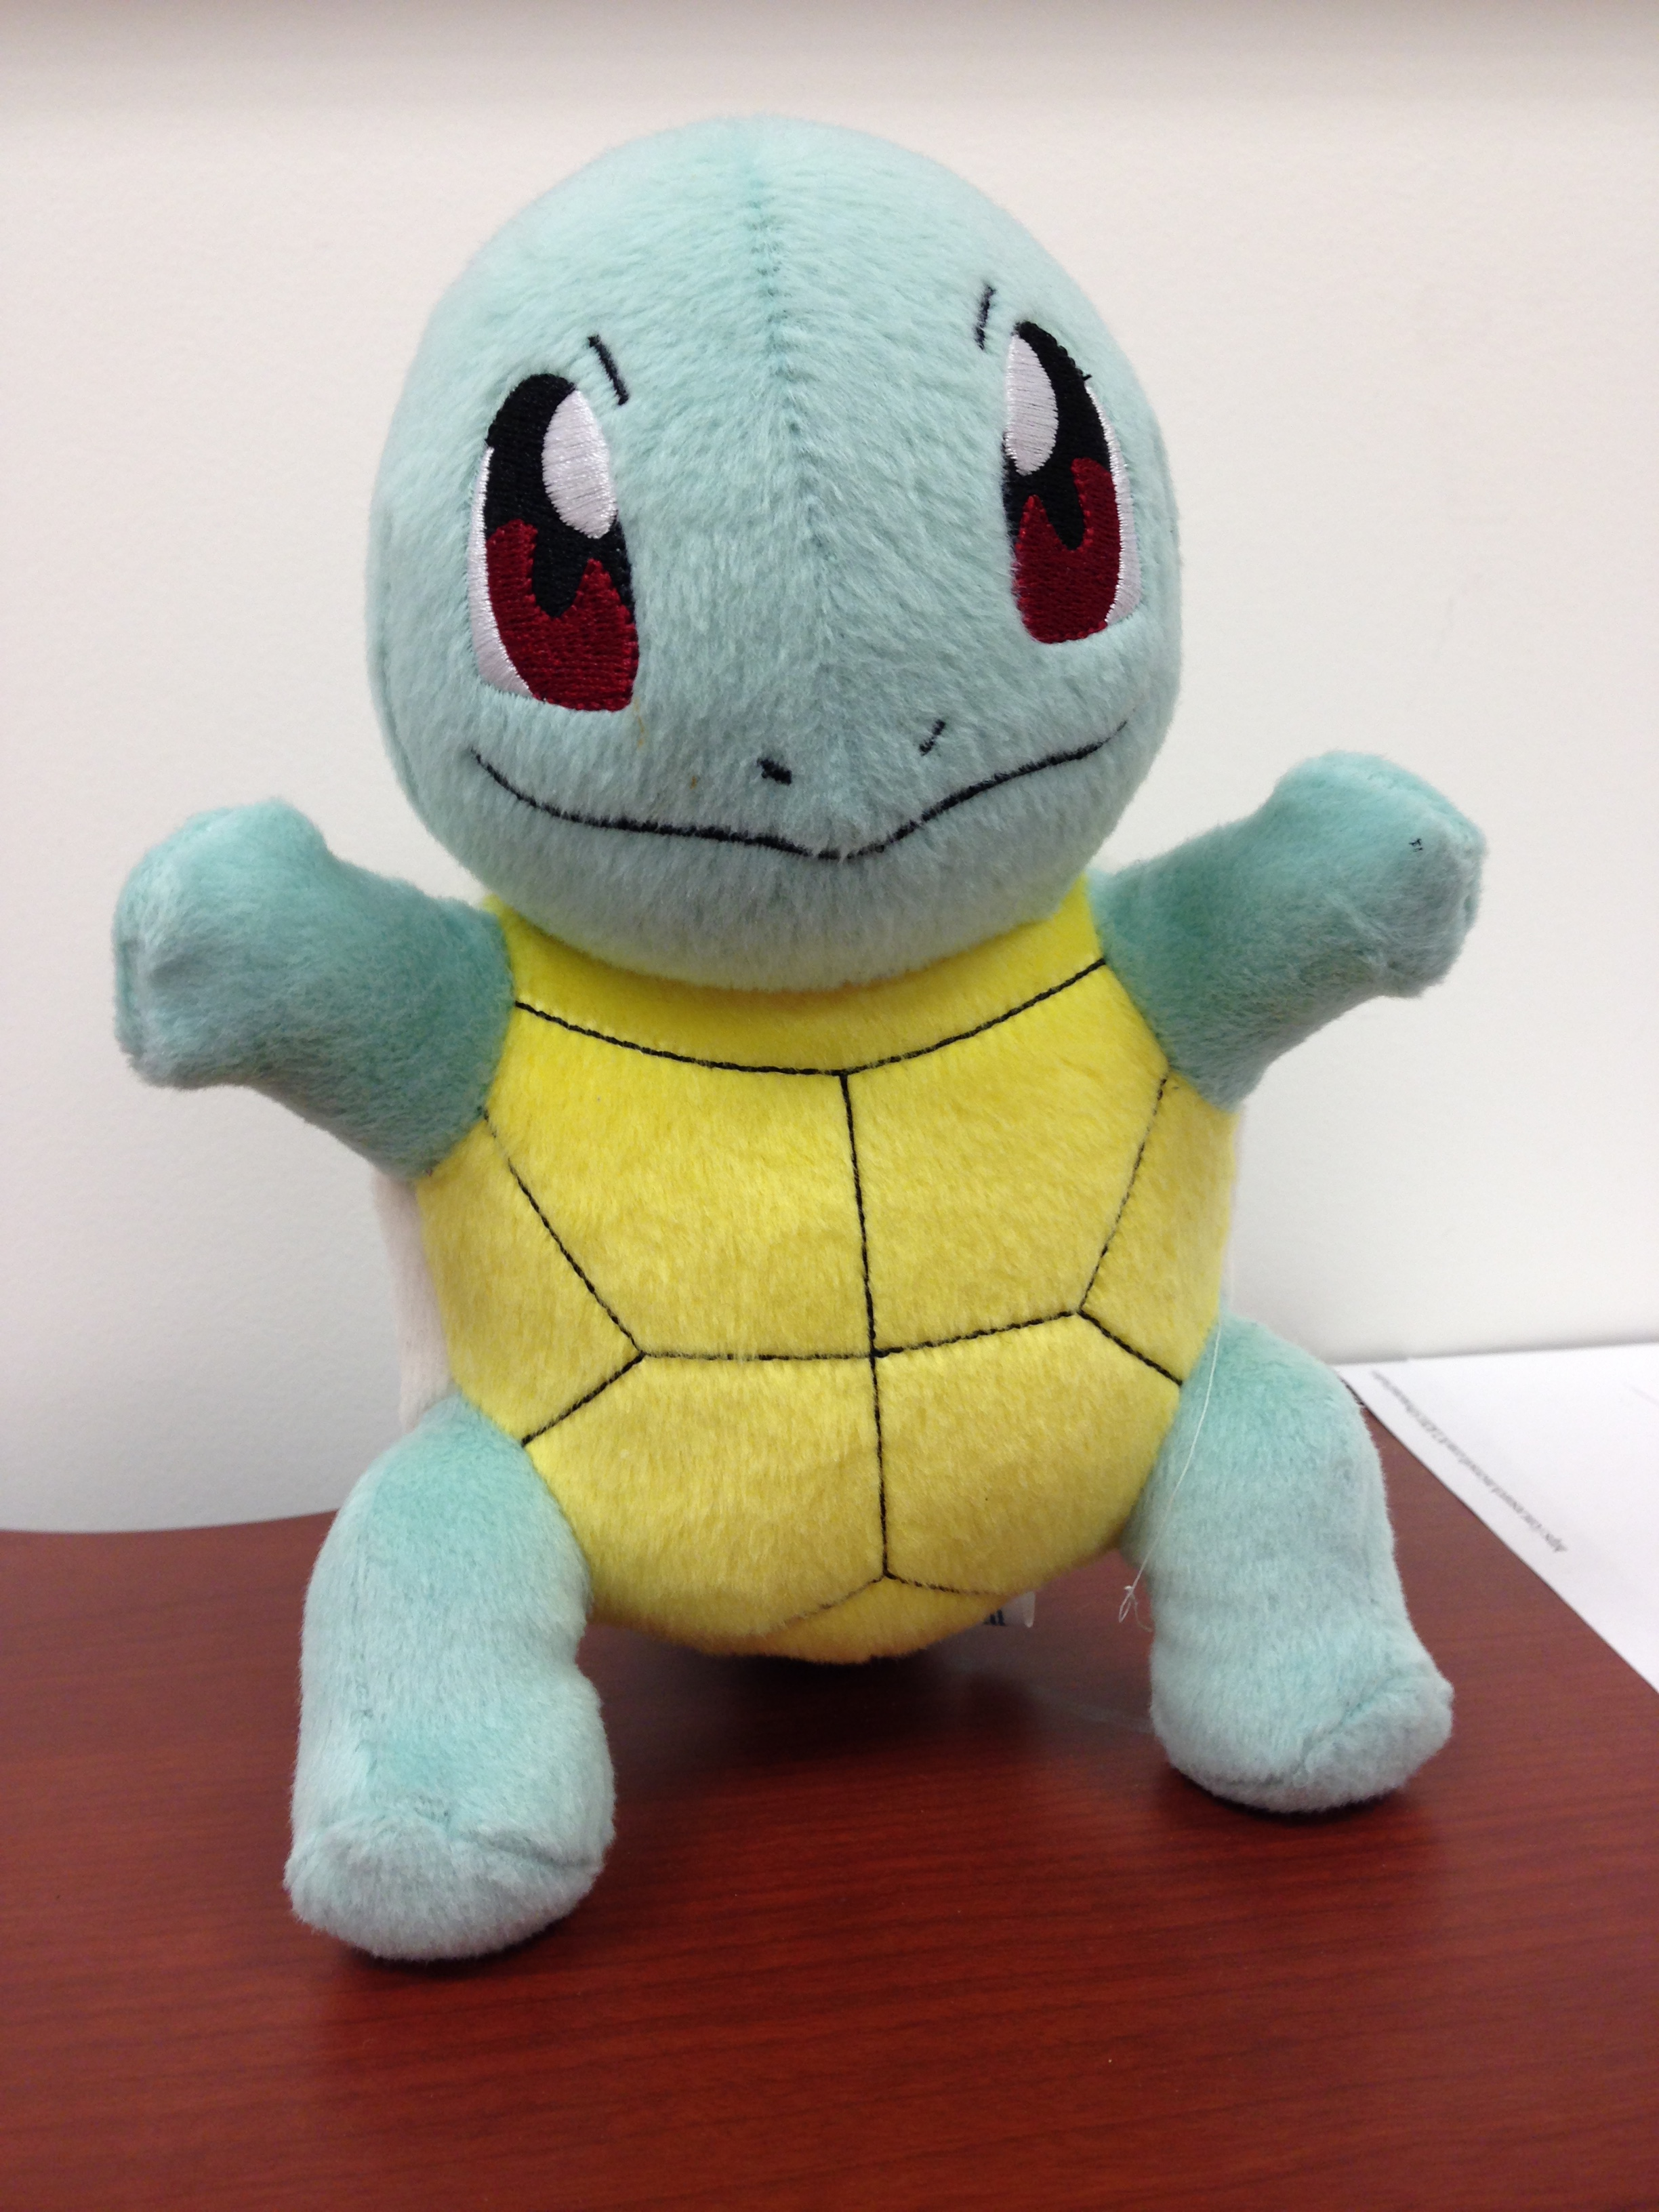
\includegraphics[width=\textwidth]{squirtle1.jpg}
		\caption{Left Image}
        \end{subfigure}
        \begin{subfigure}[b]{0.4\textwidth}
                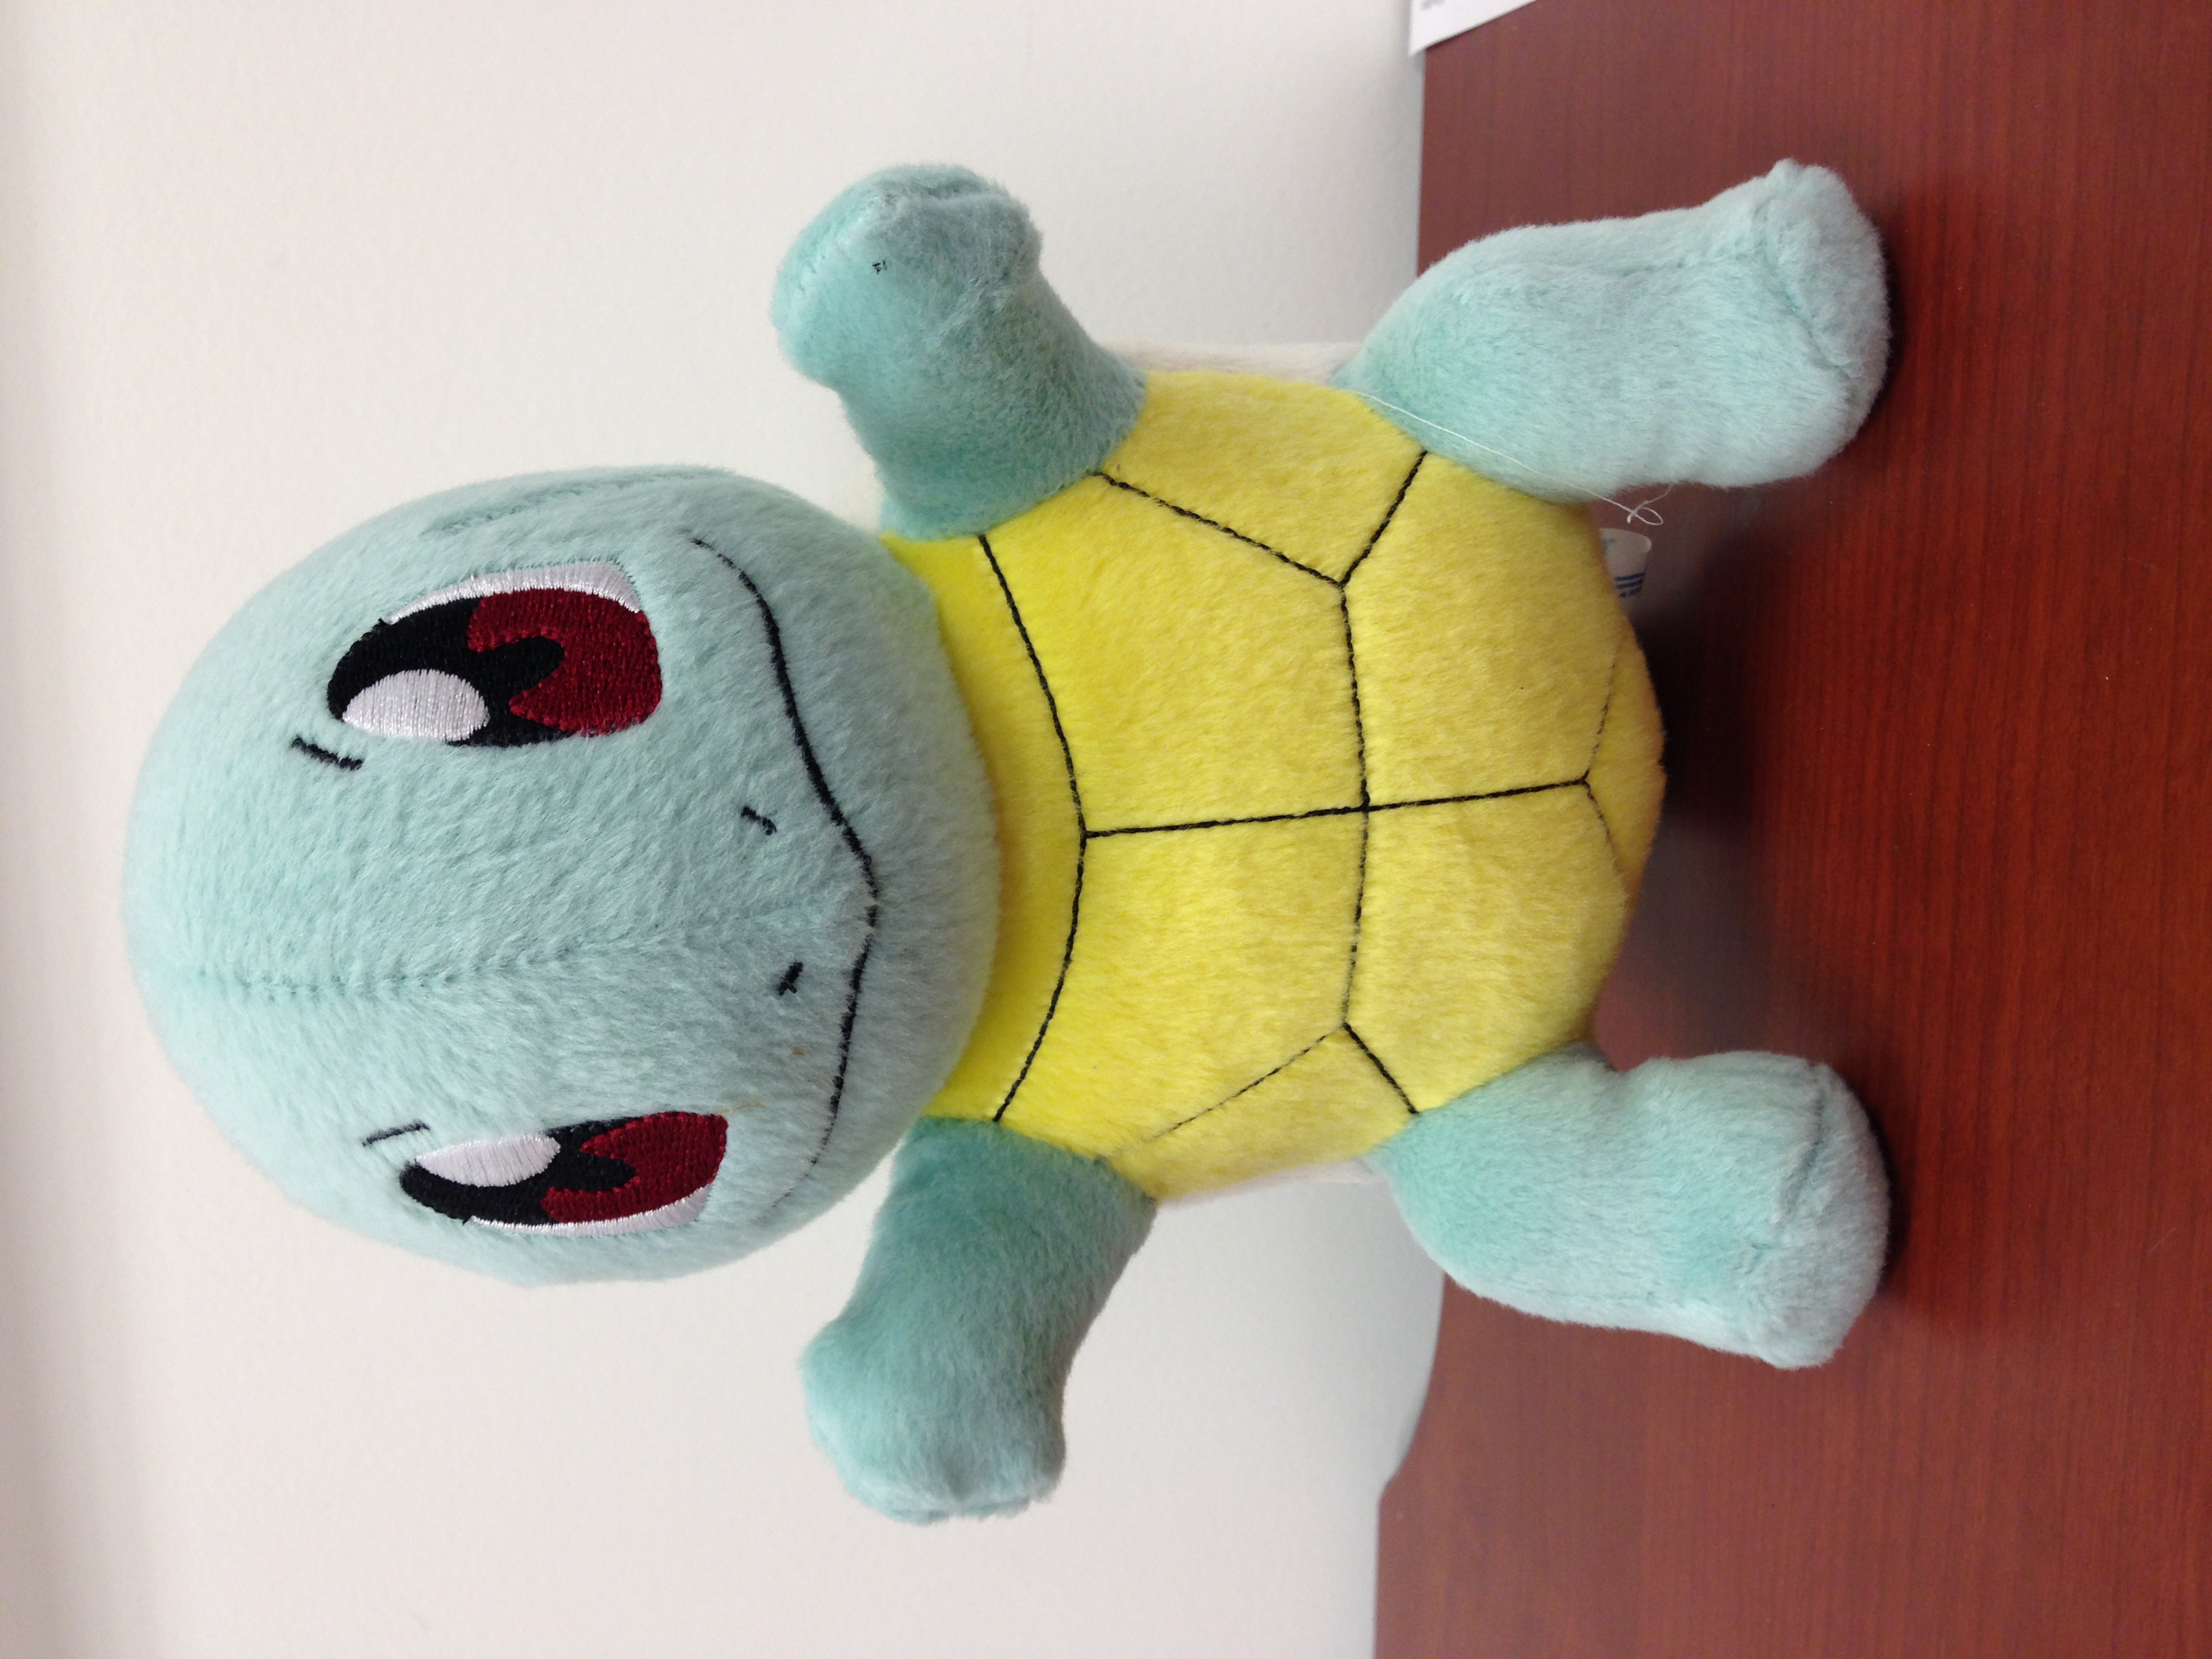
\includegraphics[width=\textwidth]{squirtle2.jpg}
                \caption{Right Image}
        \end{subfigure}
        \caption{Original Pictures of Stuffed Squirtle}
        \label{1}
\end{figure}

\begin{figure}[H]
\centering
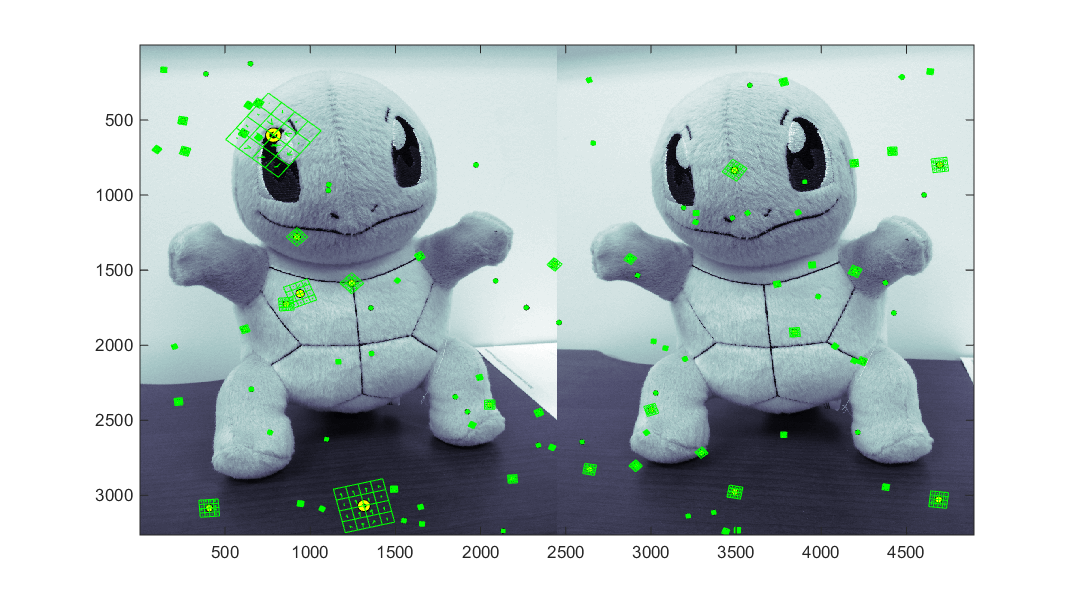
\includegraphics[height=3.5in]{squirtle_pointsWoMatching.png}
\caption{Squirtle Images With Points Marked}
\label{sq2}
\end{figure}

\begin{figure}[H]
\centering
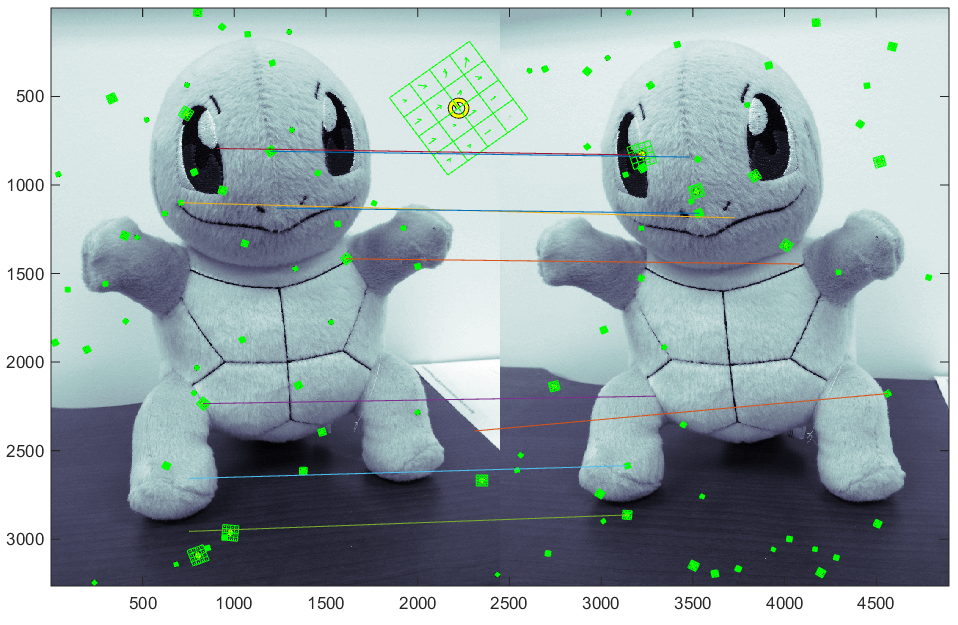
\includegraphics[height=3.5in]{squirtle_pointsWithMatching.png}
\caption{Squirtle Images With Points Marked and Some Matches Shown}
\label{sq3}
\end{figure}

\newpage

\subsection*{Book Example}

Figure 4 shows the original pictures that I took of a textbook. Figure 5 show 50 random points found by running SIFT. Figure 6 shows some of the matches found using SIFT. 

\begin{figure}
        \centering
        \begin{subfigure}[b]{0.4\textwidth}
                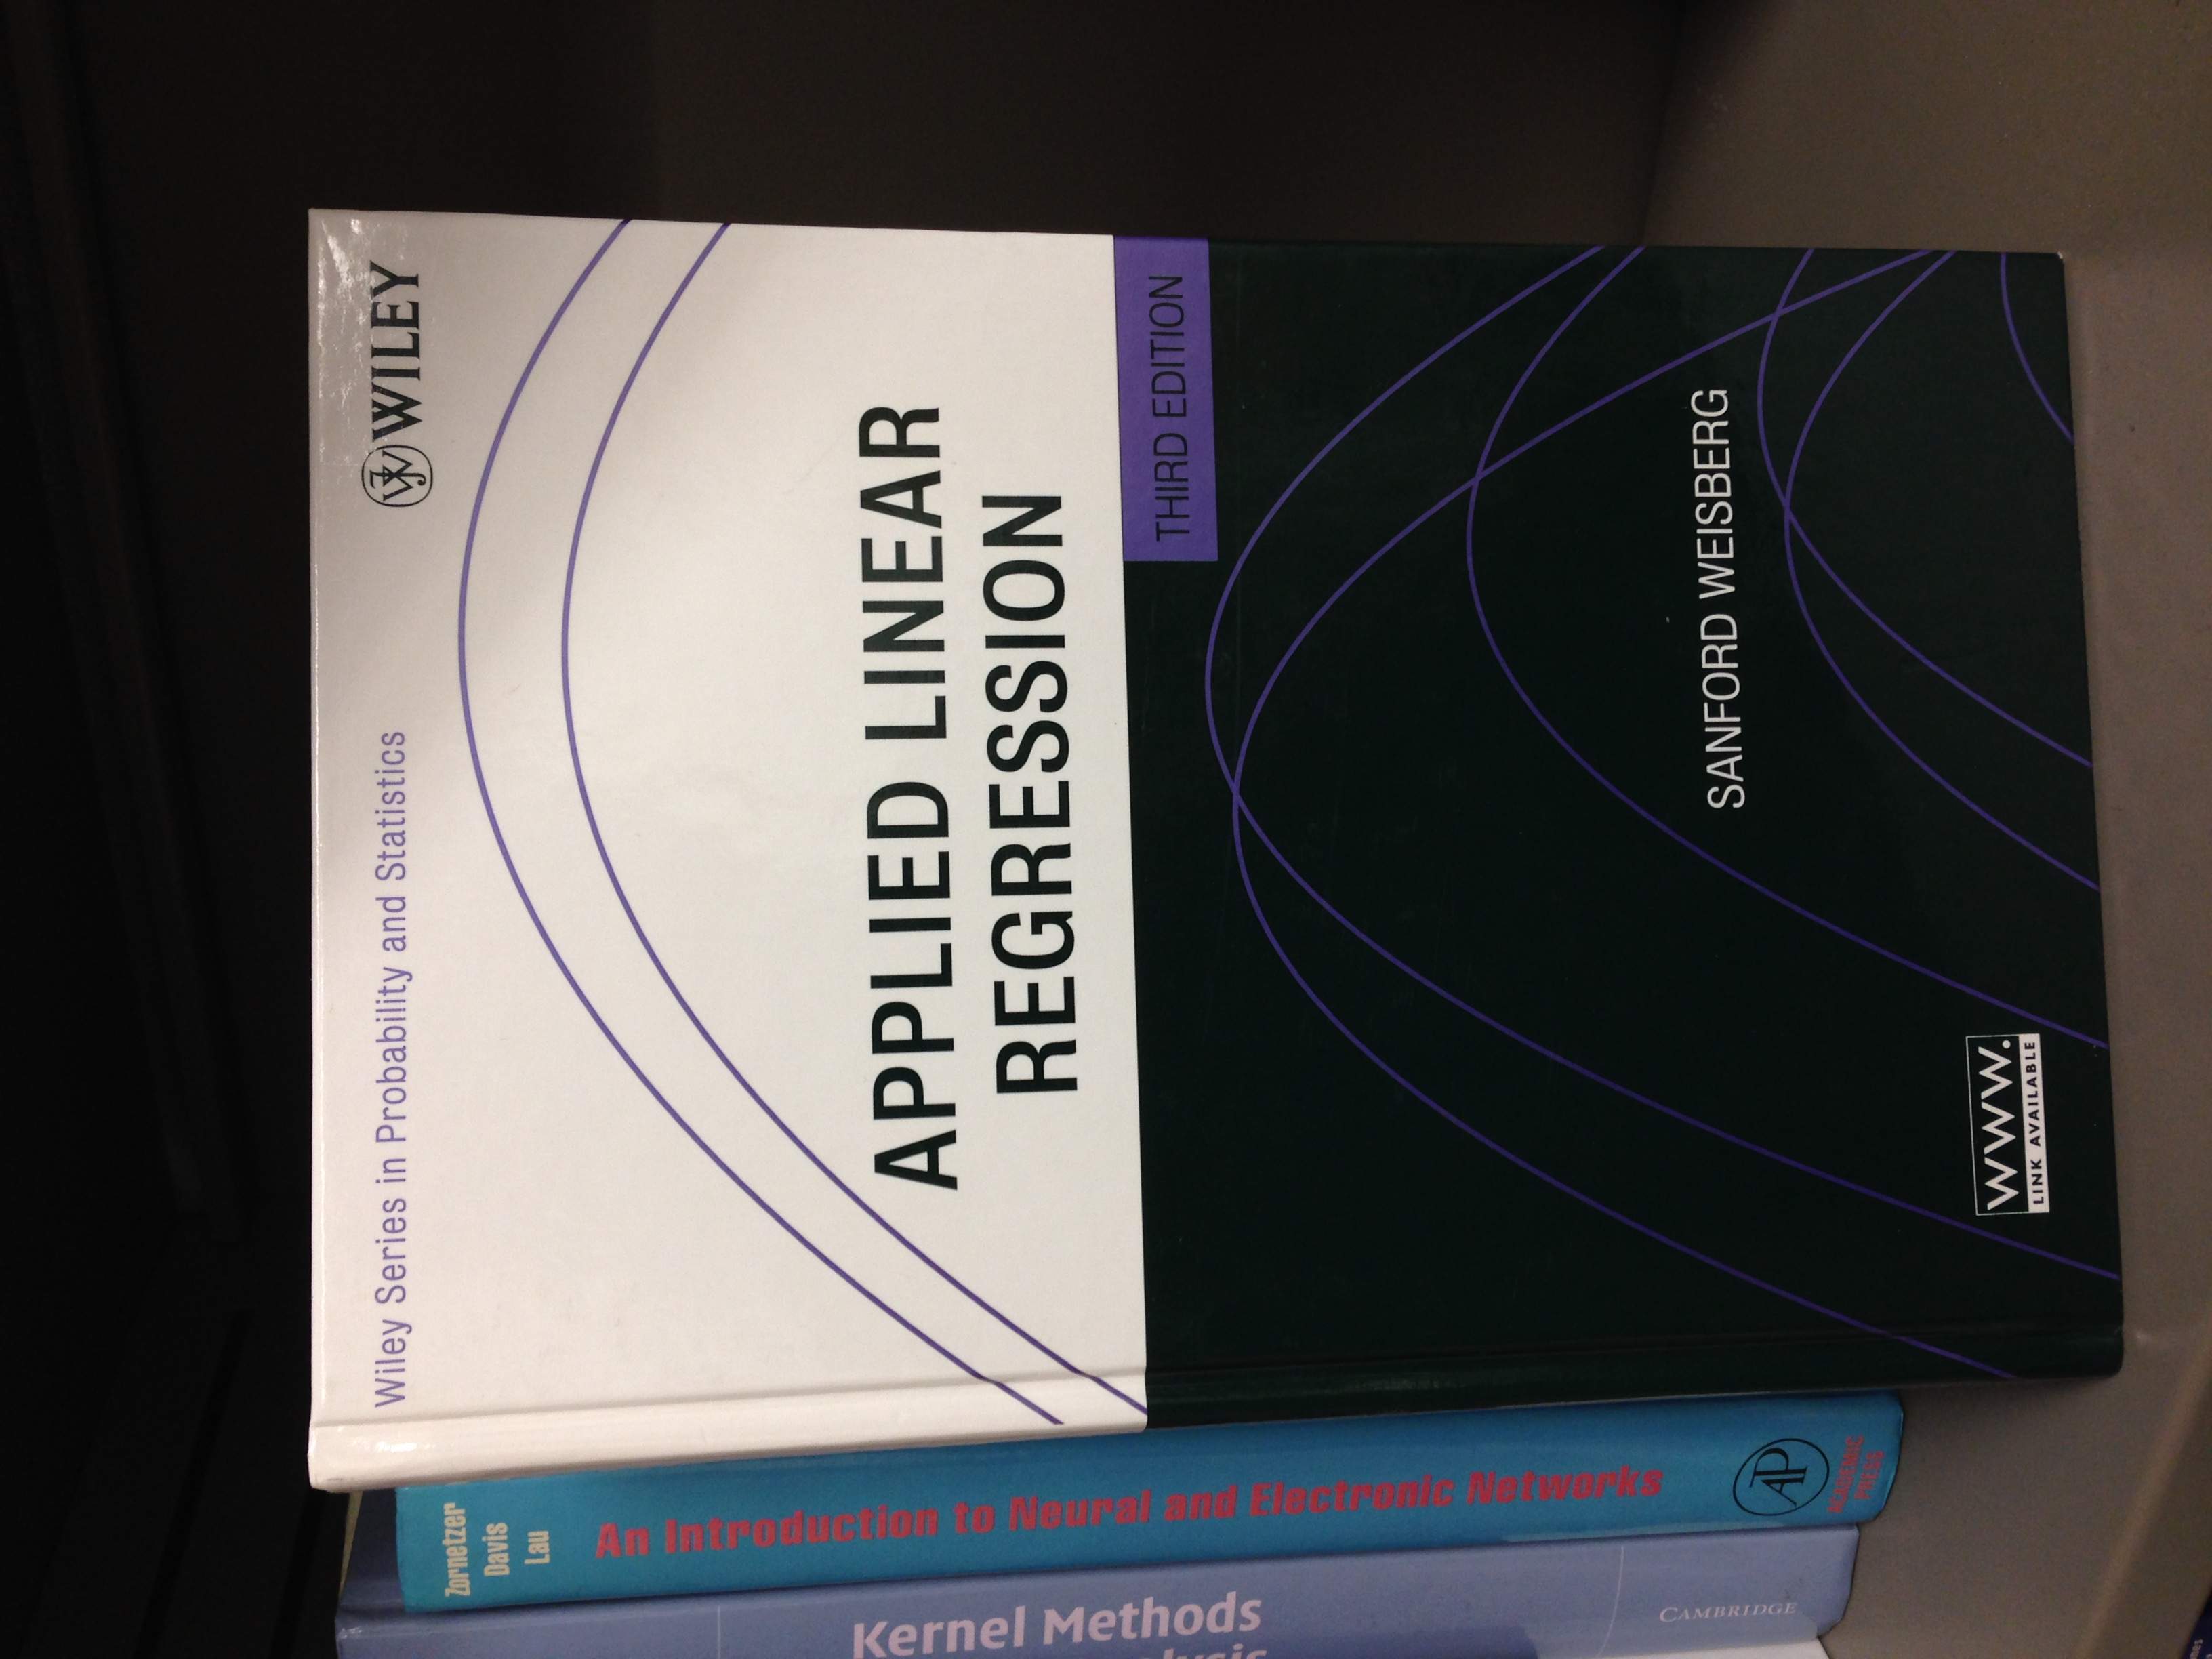
\includegraphics[width=\textwidth]{book1.jpg}
		\caption{Left Image}
        \end{subfigure}
        \begin{subfigure}[b]{0.4\textwidth}
                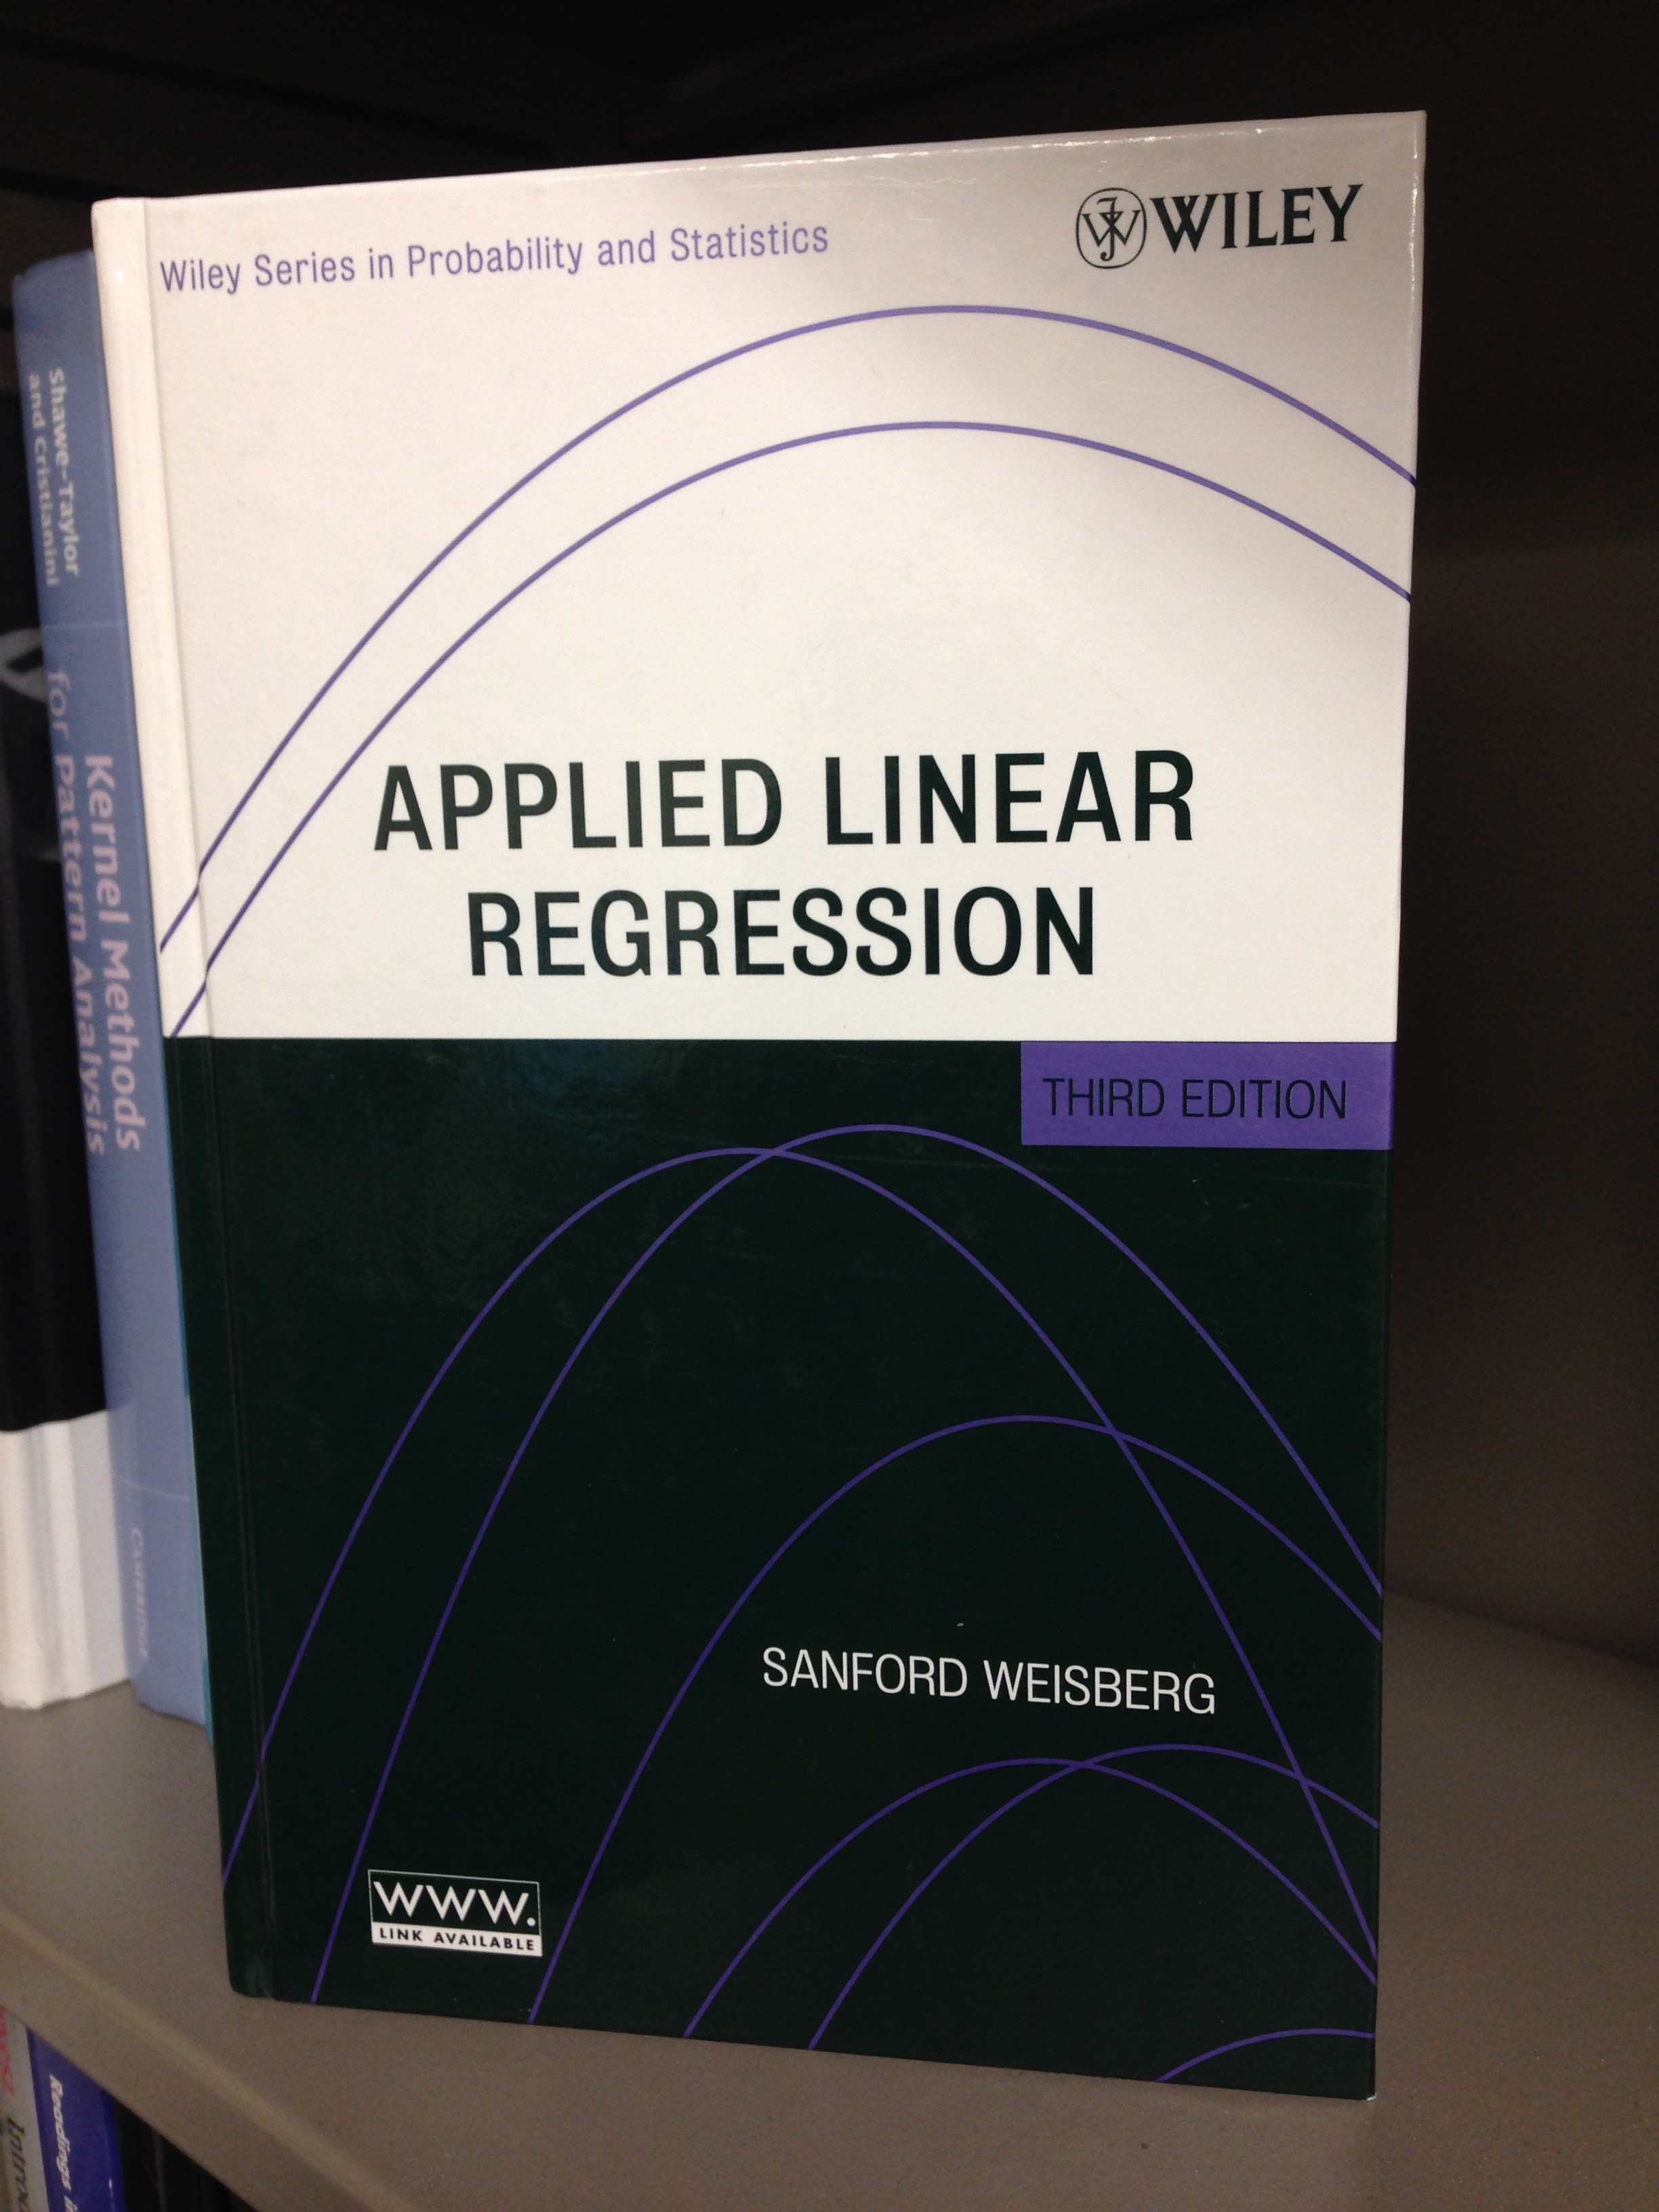
\includegraphics[width=\textwidth]{book2.jpg}
                \caption{Right Image}
        \end{subfigure}
        \caption{Original Pictures of Textbook}
        \label{bk1}
\end{figure}

\begin{figure}[H]
\centering
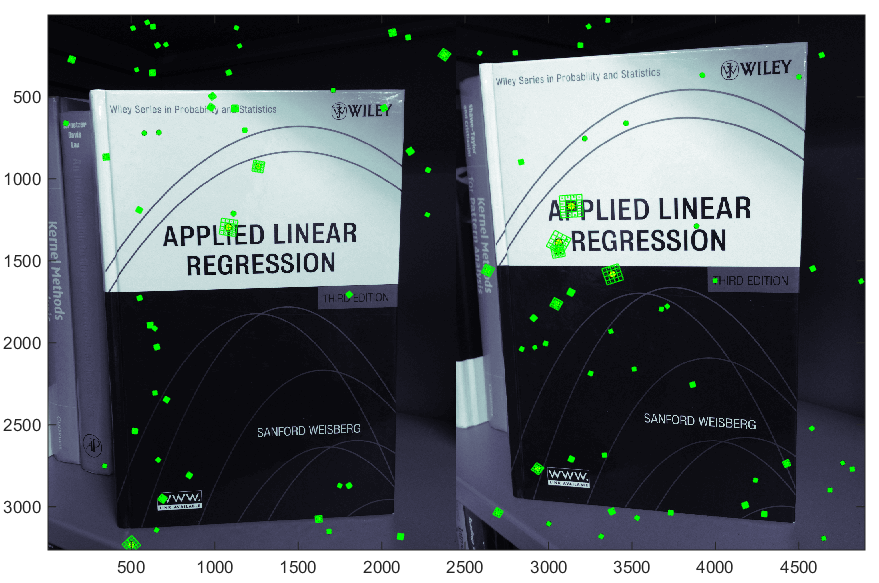
\includegraphics[height=3.5in]{book_pointsWoMatching.png}
\caption{Textbook Images With Points Marked}
\label{bk2}
\end{figure}

\begin{figure}[H]
\centering
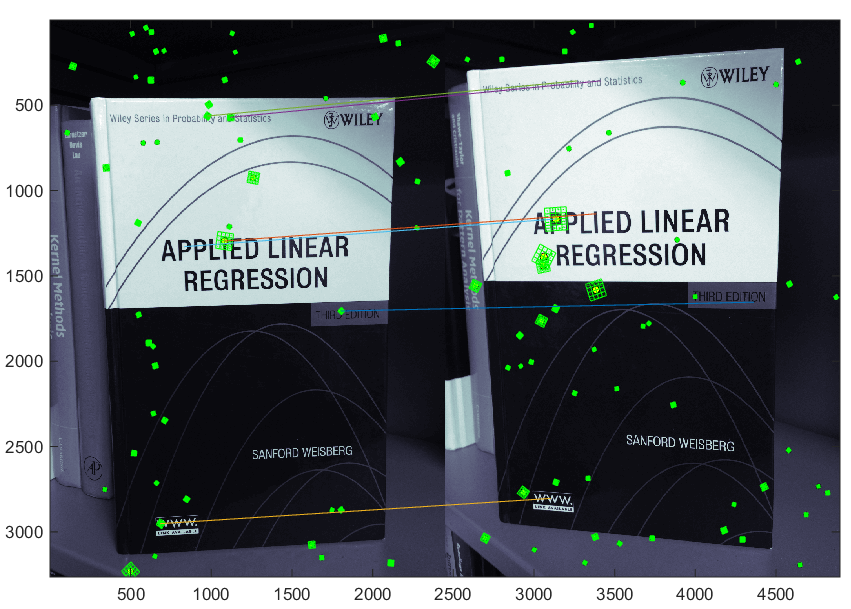
\includegraphics[height=3.5in]{book_pointsWithMatching.png}
\caption{Textbook Images With Points Marked and Some Matches Shown}
\label{bk3}
\end{figure}

\newpage

\subsection*{Coffee Can Example}

Figure 7 shows the original pictures that I took of a coffee can. Figure 8 show 50 random points found by running SIFT. Figure 9 shows some of the matches found using SIFT. 

\begin{figure}
        \centering
        \begin{subfigure}[b]{0.4\textwidth}
                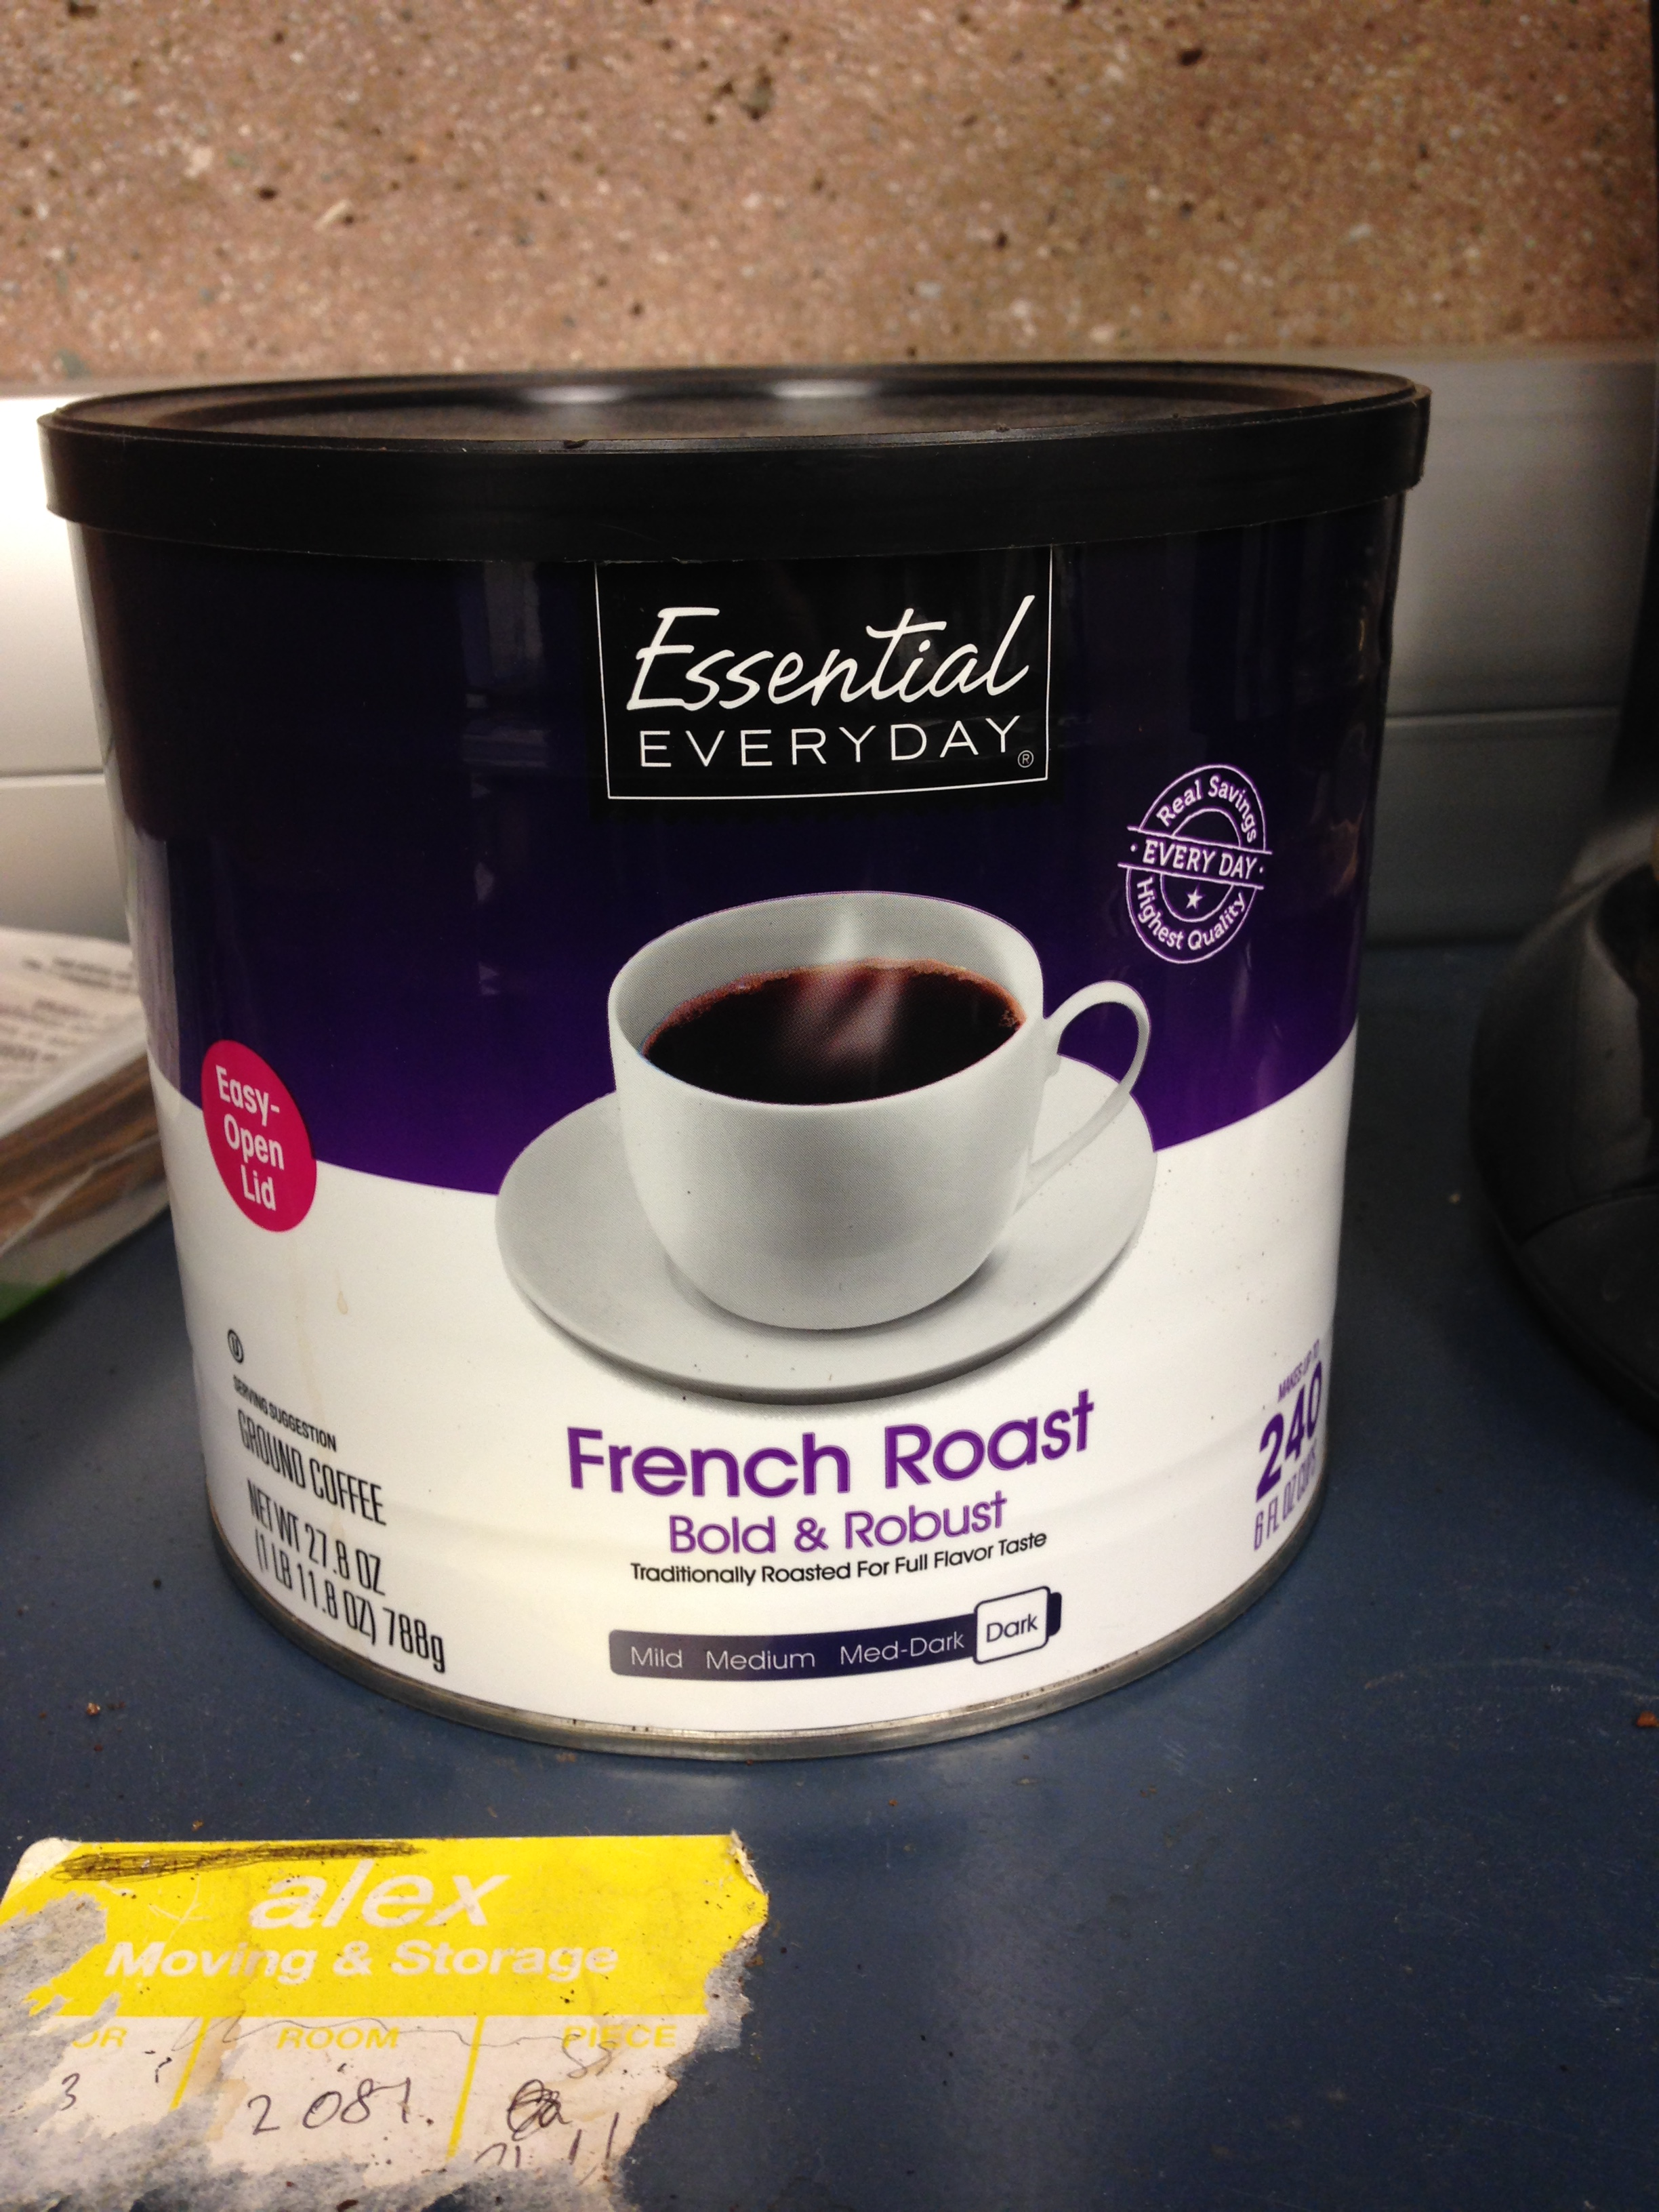
\includegraphics[width=\textwidth]{coffeeCan1.jpg}
		\caption{Left Image}
        \end{subfigure}
        \begin{subfigure}[b]{0.4\textwidth}
                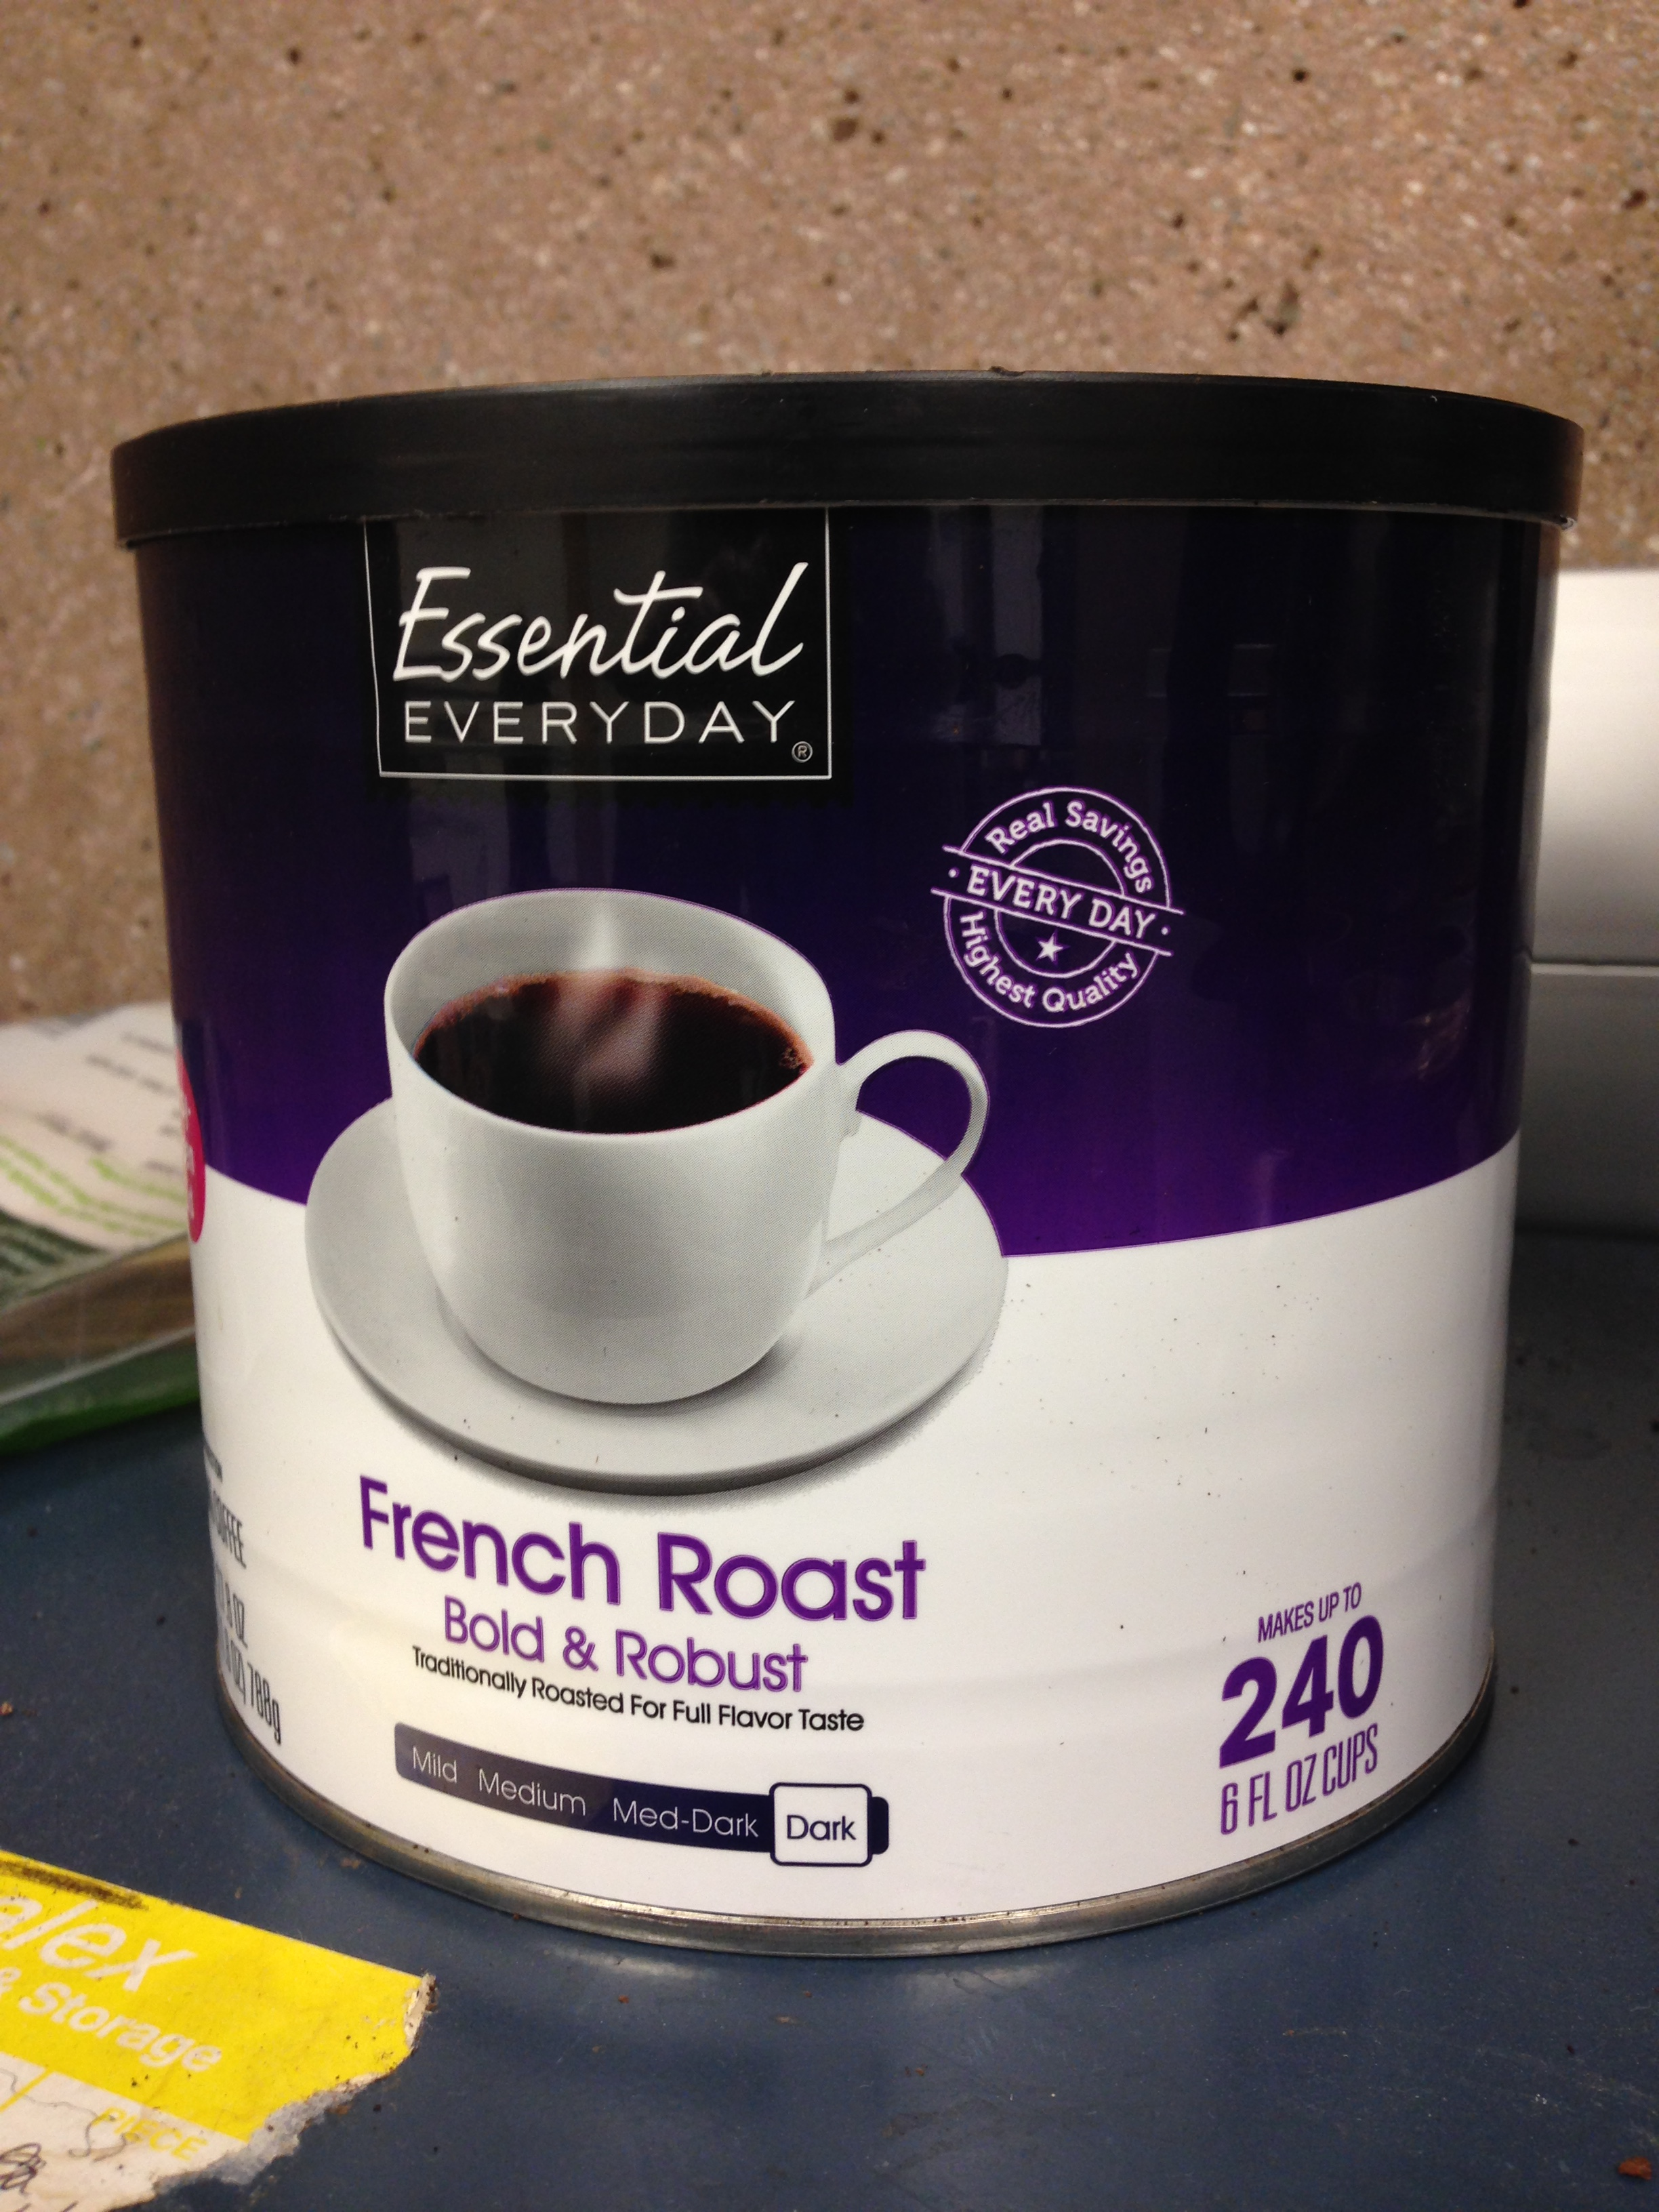
\includegraphics[width=\textwidth]{coffeeCan2.jpg}
                \caption{Right Image}
        \end{subfigure}
        \caption{Original Pictures of Coffee Can}
        \label{cc1}
\end{figure}

\begin{figure}[H]
\centering
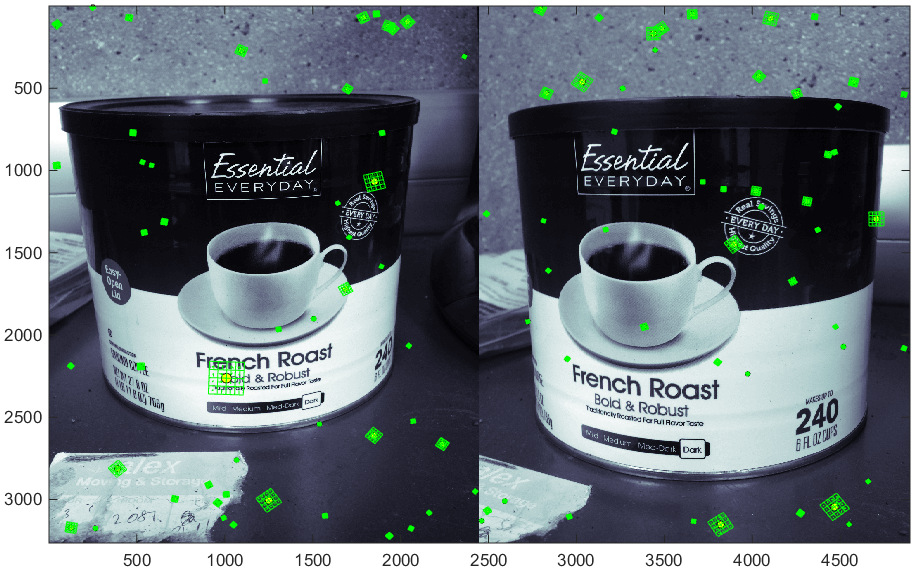
\includegraphics[height=3.5in]{coffeeCan_pointsWoMatching.png}
\caption{Coffee Can Images With Points Marked}
\label{cc2}
\end{figure}

\begin{figure}[H]
\centering
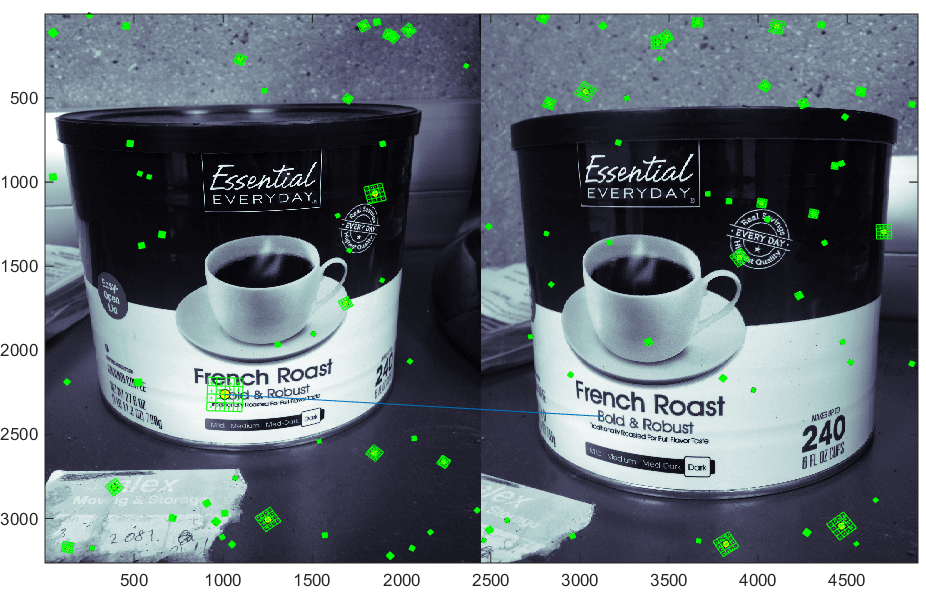
\includegraphics[height=3.5in]{coffeeCan_pointsWithMatching.png}
\caption{Coffee Can Images With Points Marked and Some Matches Shown}
\label{cc3}
\end{figure}

\subsection*{Code for Problem 1}

The code for this problem is in the folder as prob1script.m

\newpage

\section*{Problem 2}

For problem 2, I used the same images as the previous problem and I used points chosen by myself as well as points chosen through SIFT. The first part of this write-up shows the results when I used my own parts. The second part of the write up shows the results when I used the points found through SIFT. With my own points, I made sure they were selected in the same order in both images so the matches had the same index. With the SIFT points, I used the matching results from running ubcmatch. In both cases, I decided to test each matching pair using RANSAC in order to get a final set of pairs. 

\subsection*{Part A, My Points}

Figures 10, 11, and 12 show the points that I chose in each image. After running my own implementation of RANSAC, I got the correspondences that are shown in figures 13, 14, and 15.

\begin{figure}[H]
\centering
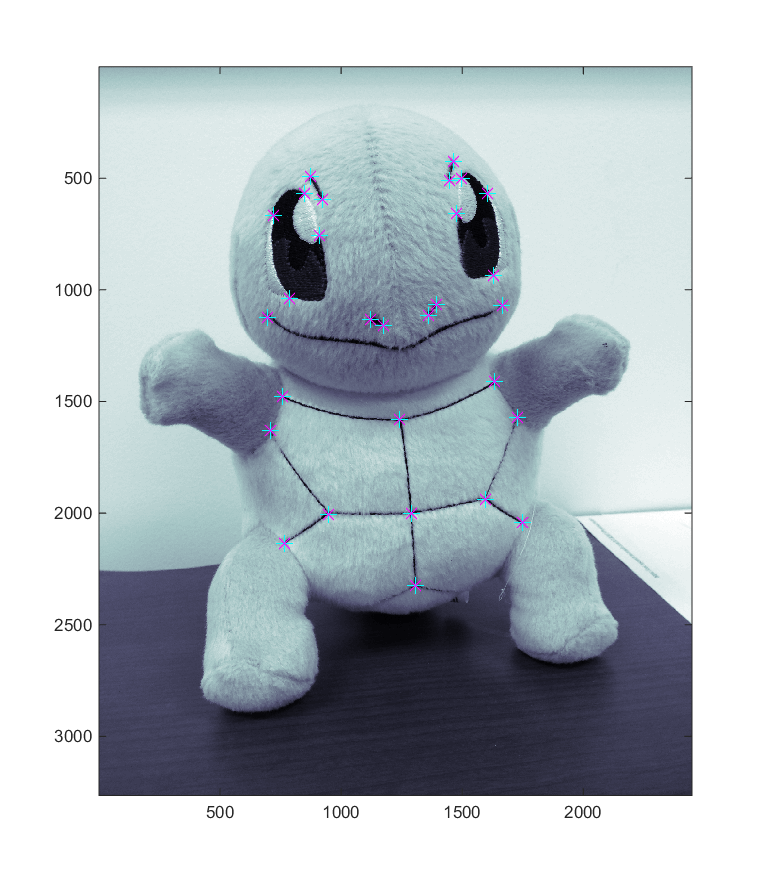
\includegraphics[height=7in]{squirtle_prob2Points.png}
\caption{Squirtle Image with Points Marked}
\label{p2a}
\end{figure}

\begin{figure}[H]
\centering
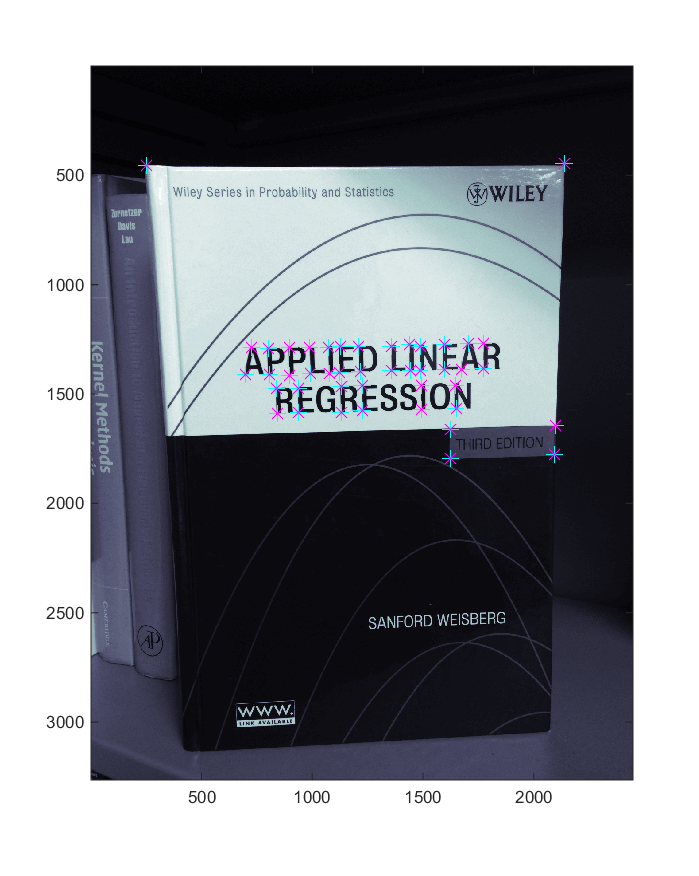
\includegraphics[height=7in]{book_prob2Points.png}
\caption{Textbook Image with Points Marked}
\label{p2b}
\end{figure}

\begin{figure}[H]
\centering
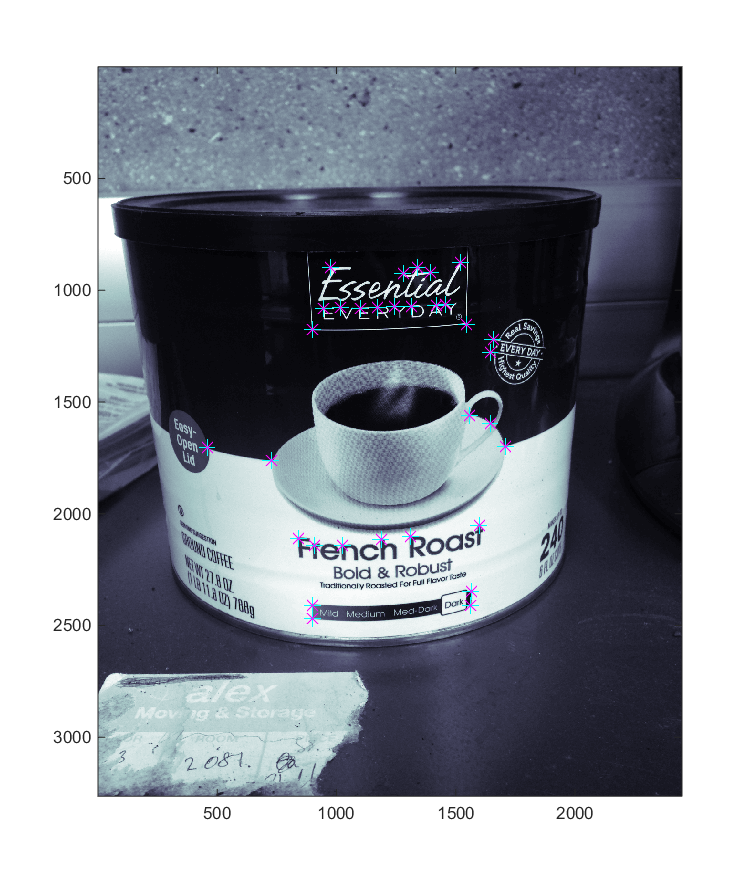
\includegraphics[height=7in]{coffeeCan_prob2Points.png}
\caption{Coffee Can Image with Points Marked}
\label{p2c}
\end{figure}

\begin{figure}[H]
\centering
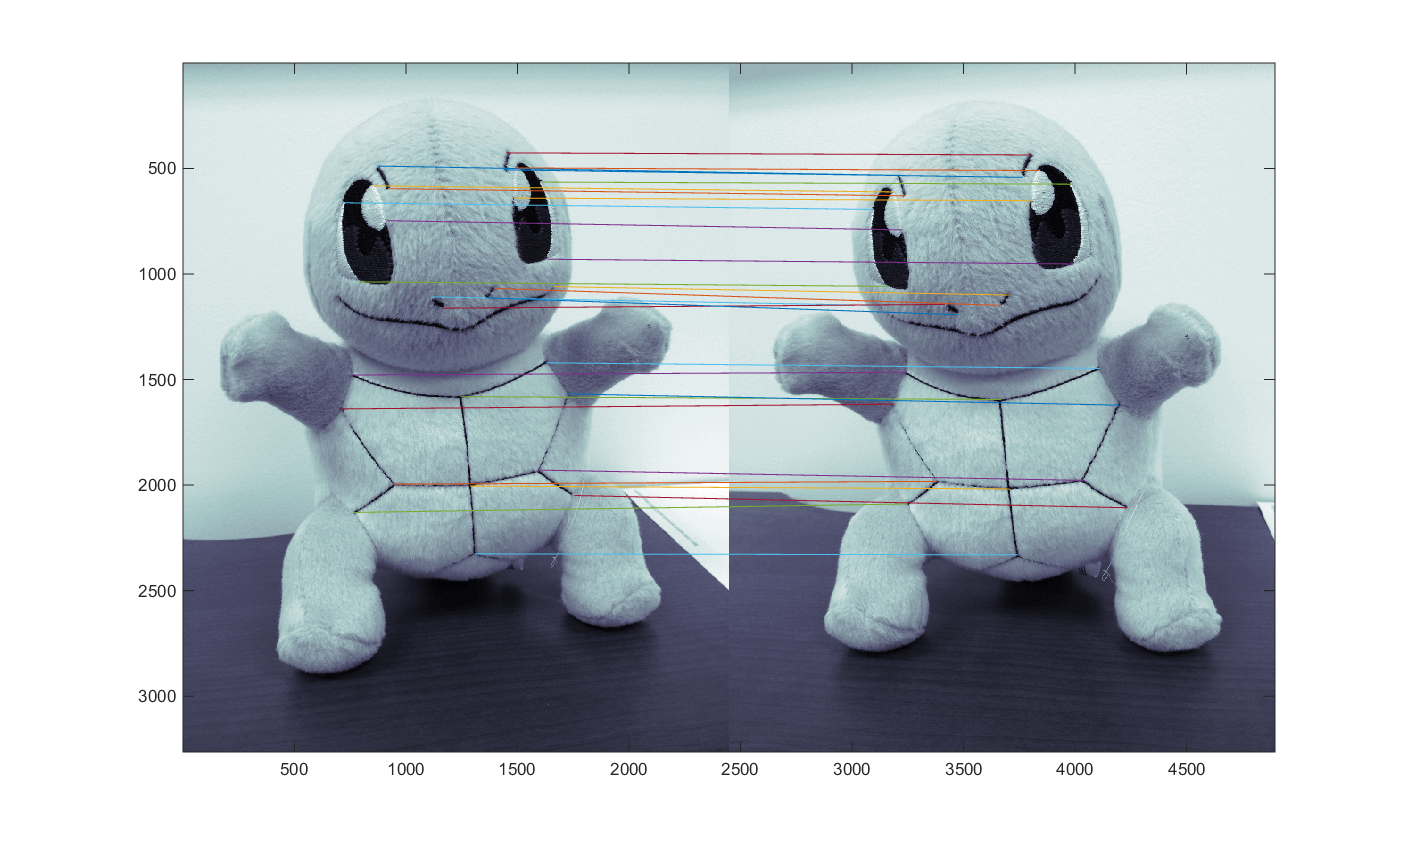
\includegraphics[height=4.5in]{squirtle_prob2Matches.png}
\caption{Squirtle Images with matching points}
\label{p2d}
\end{figure}

\begin{figure}[H]
\centering
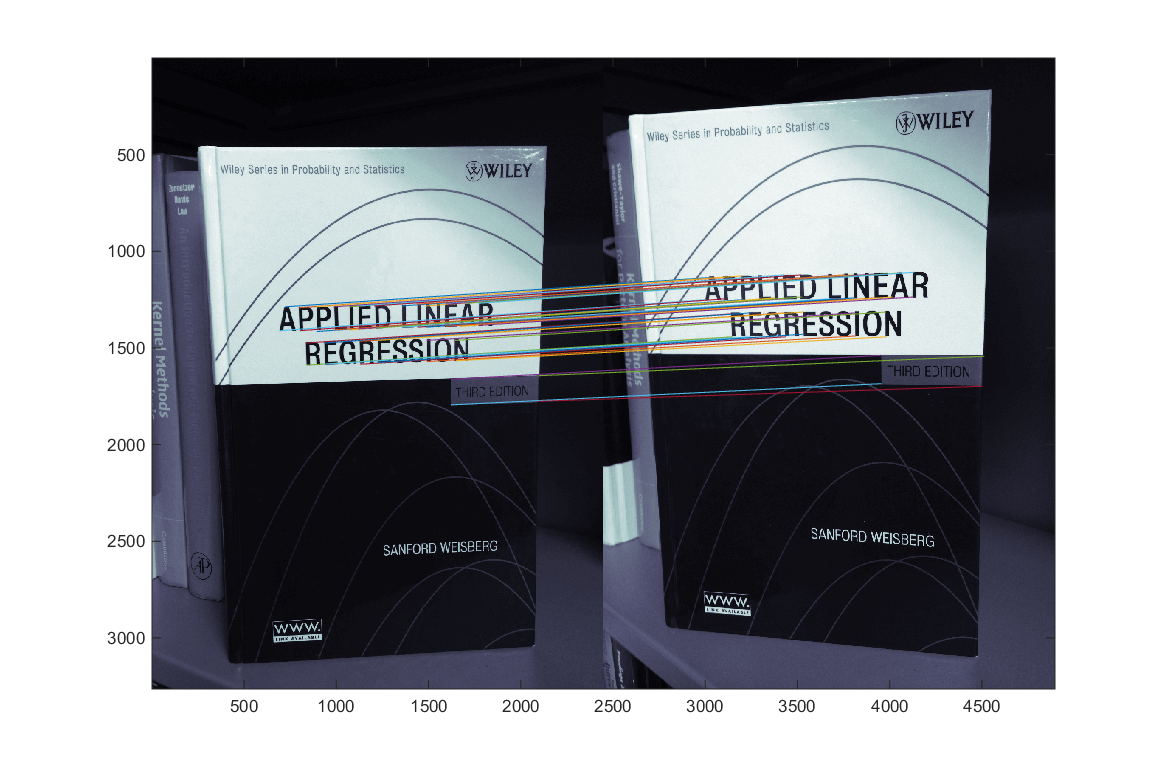
\includegraphics[height=5in]{book_prob2Matches.png}
\caption{Textbook Images with matching points}
\label{p2e}
\end{figure}

\begin{figure}[H]
\centering
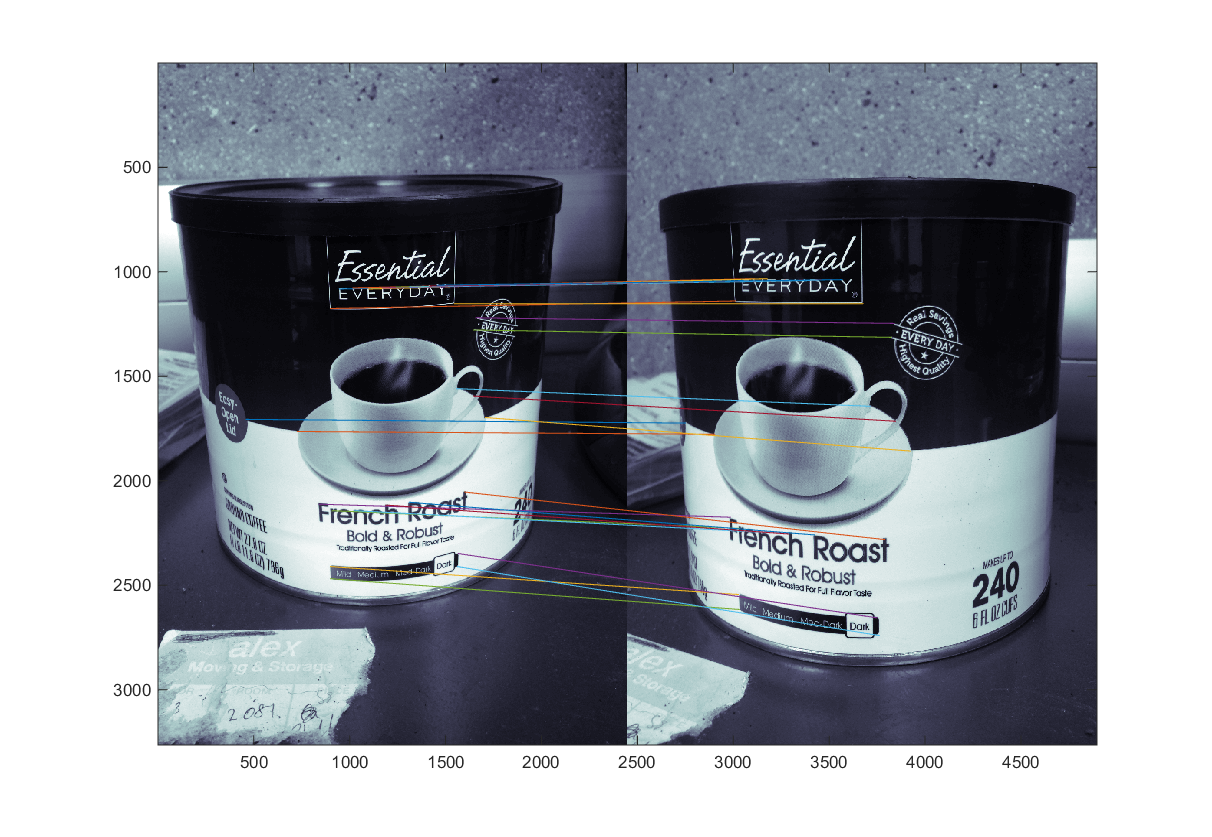
\includegraphics[height=5in]{coffeeCan_prob2Matches.png}
\caption{Coffee Can Images with matching points}
\label{p2f}
\end{figure}

\newpage

\subsection*{Part B, My Points}

With the squirtle image, the epipole for the left image lies slightly above the epipole for the right image, suggesting that the left image was taken from a slightly raised viewpoint as compared to the right image. With the coffee can image, the epipole of the left image is below the epipole for right image, suggesting that it was taken from a lowered viewpoint. 

\begin{figure}[H]
\centering
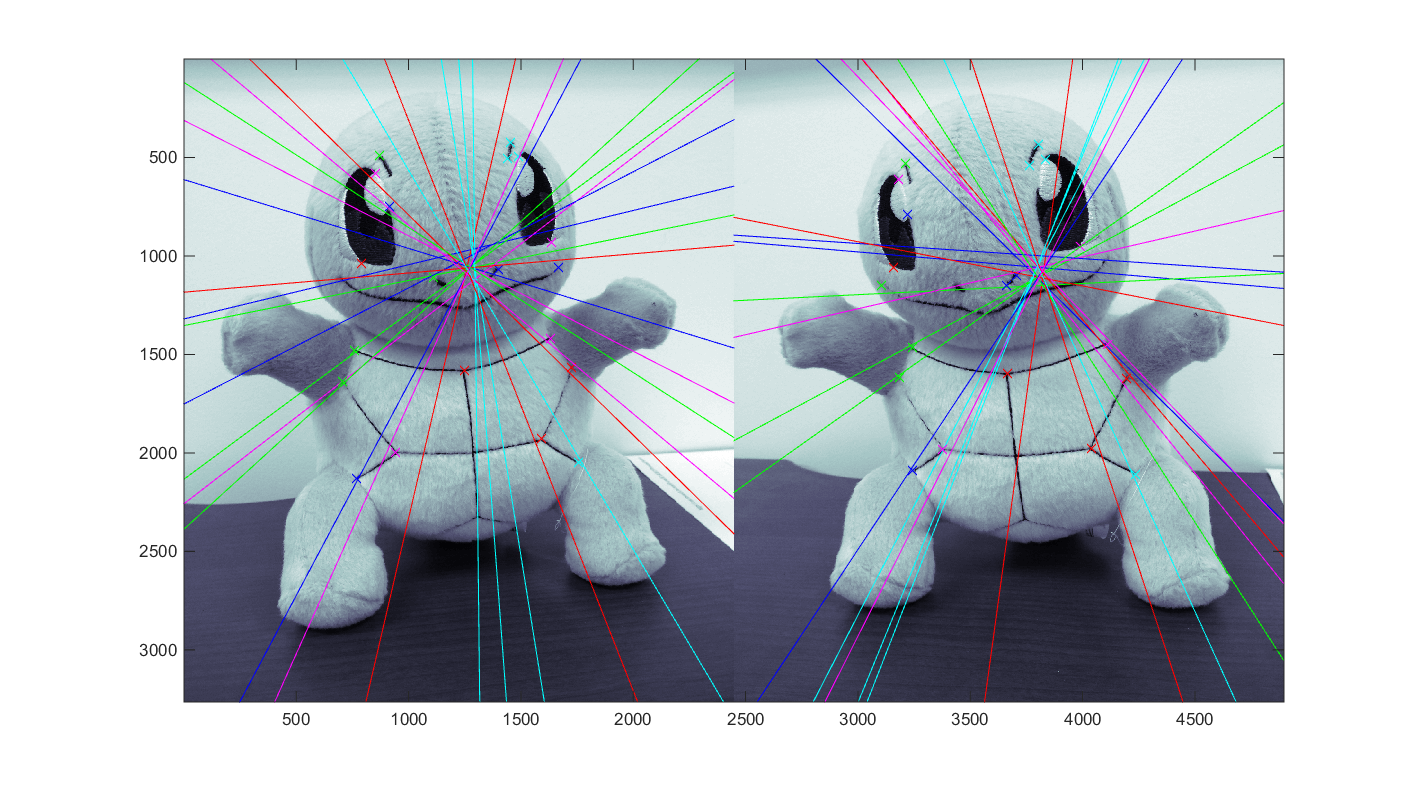
\includegraphics[height=3.5in]{squirtle_prob2Epipolar.png}
\caption{Squirtle Image with Epipolar Lines and their points}
\label{p2g}
\end{figure}

\begin{figure}[H]
\centering
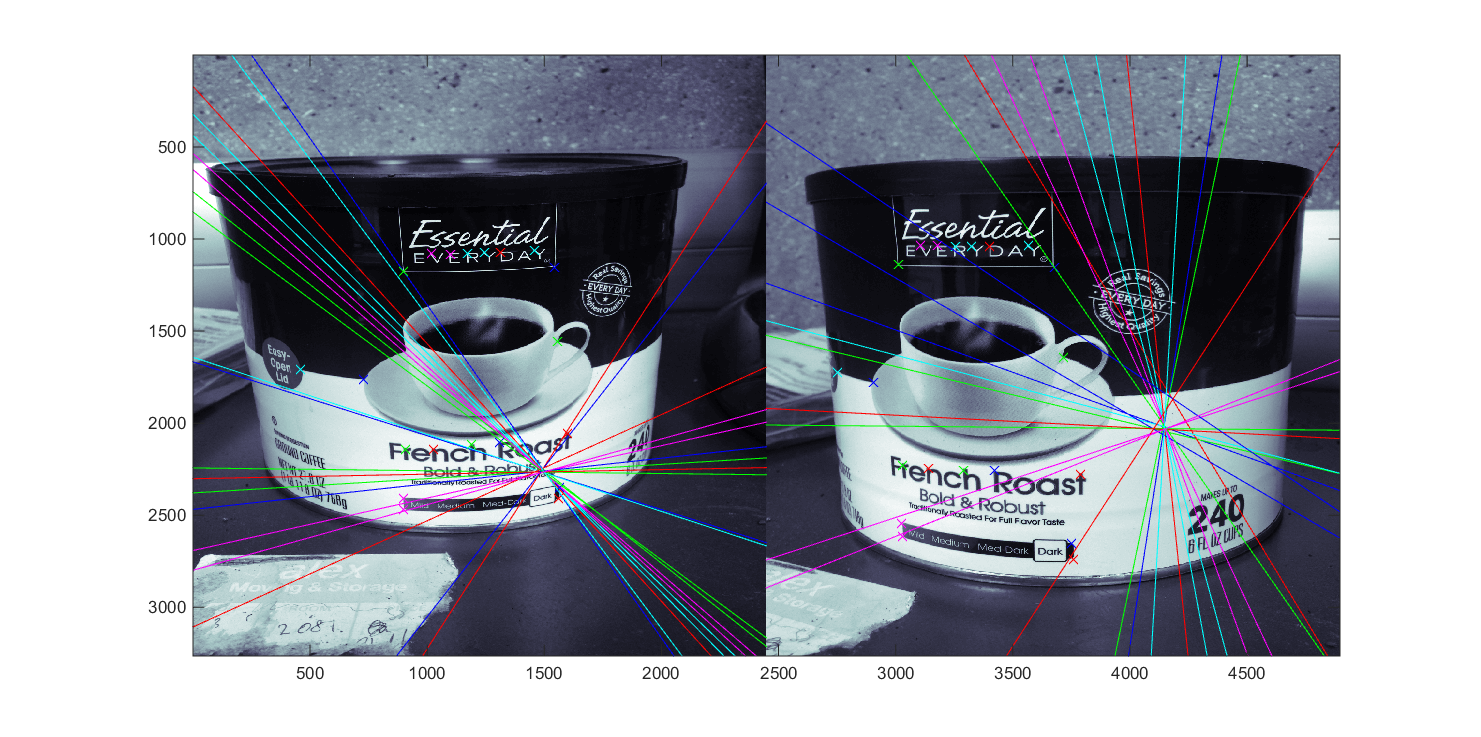
\includegraphics[height=3.5in]{coffeeCan_prob2Epipolar.png}
\caption{Coffee Can Image with Epipolar Lines and their points}
\label{p2h}
\end{figure}

\newpage

\subsection*{Part C, My Points}

The estimate for F is quite stable. I decided to compute it multiple times and find the standard deviation of the entries in the F matrix. I then summed the standard deviation. \\
\\
For squirtle, the sum was near zero and 4 computations of the F matrix were done.\\
For the textbook, the sum was 0.9567 and 6 computations of the F matrix were done.\\
For the coffee can, the sum was 1.0140 and 6 computations of the F matrix were done. \\
\\
The best way to make F more robust would have been to add more points and then see if they correspond. With more data, the estimates get more robust. 

\subsection*{Part A, SIFT points}

Figures 18, 19, and 20 show the points chosen by SIFT in each image. I then ran my own implementation of RANSAC and only used the SIFT pairs that matched well. Afterwards, I got the correspondences that are shown in figures 21, 22, and 23.

\begin{figure}[H]
\centering
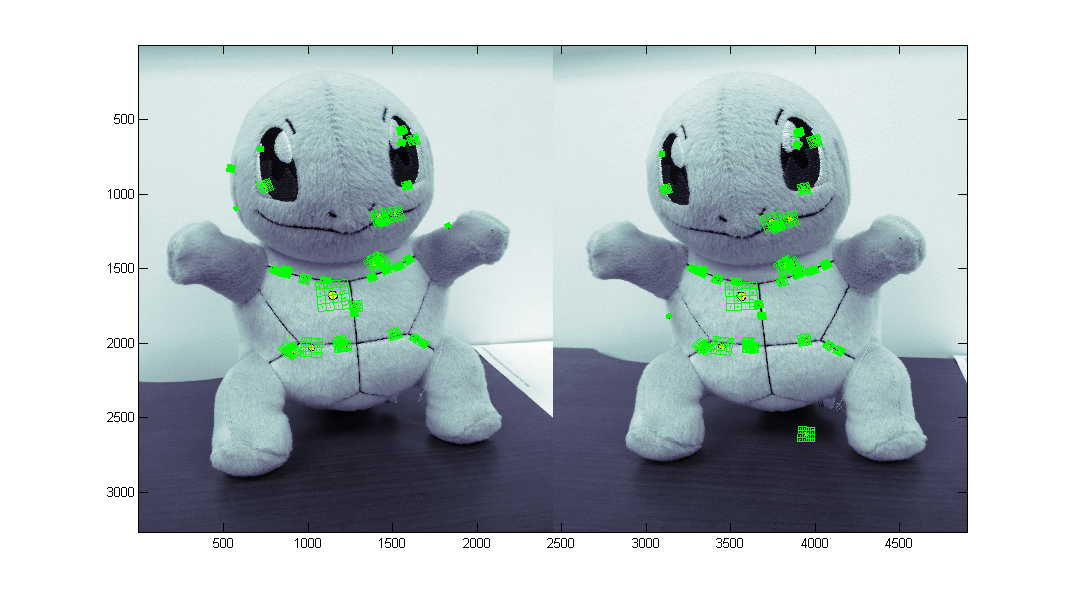
\includegraphics[height=4.5in]{squirtle_prob2Points2.png}
\caption{Squirtle Image with Points Marked}
\label{p2a}
\end{figure}

\begin{figure}[H]
\centering
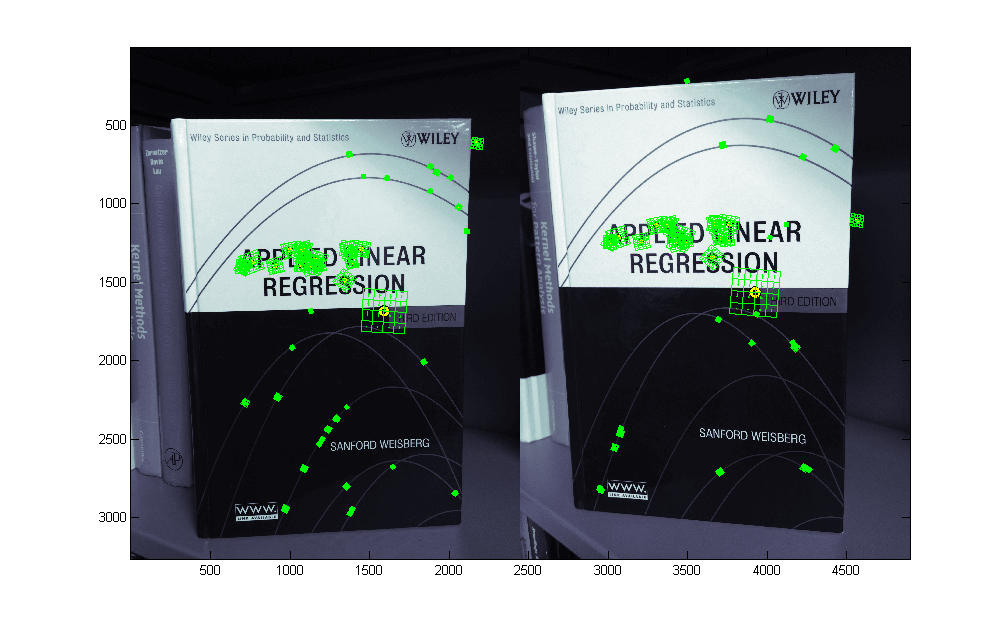
\includegraphics[height=4.5in]{book_prob2Points2.png}
\caption{Textbook Image with Points Marked}
\label{p2b}
\end{figure}

\begin{figure}[H]
\centering
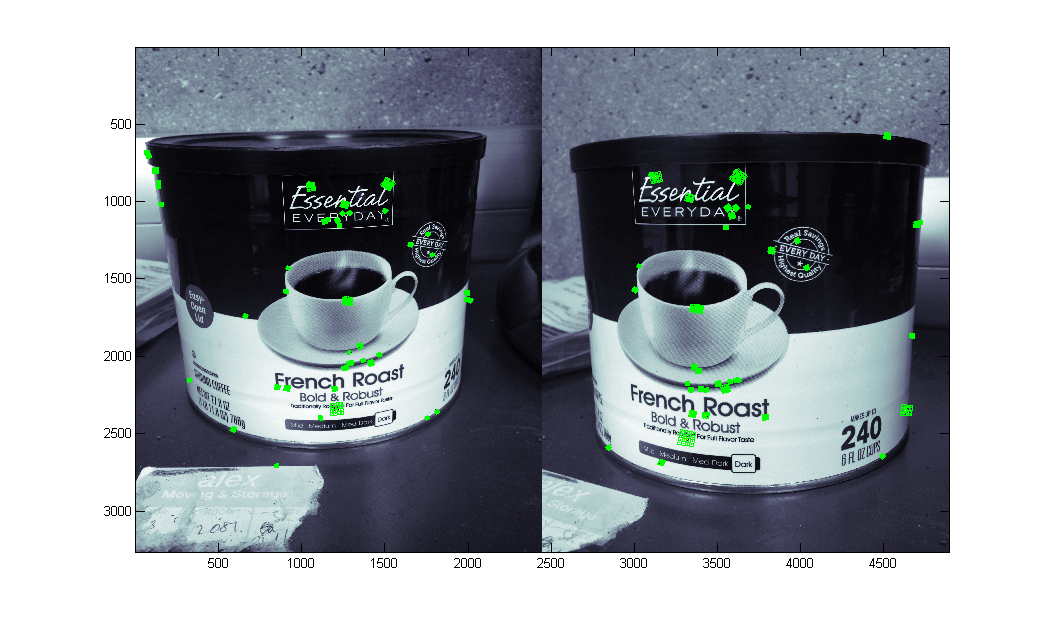
\includegraphics[height=4.5in]{coffeeCan_prob2Points2.png}
\caption{Coffee Can Image with Points Marked}
\label{p2c}
\end{figure}

\begin{figure}[H]
\centering
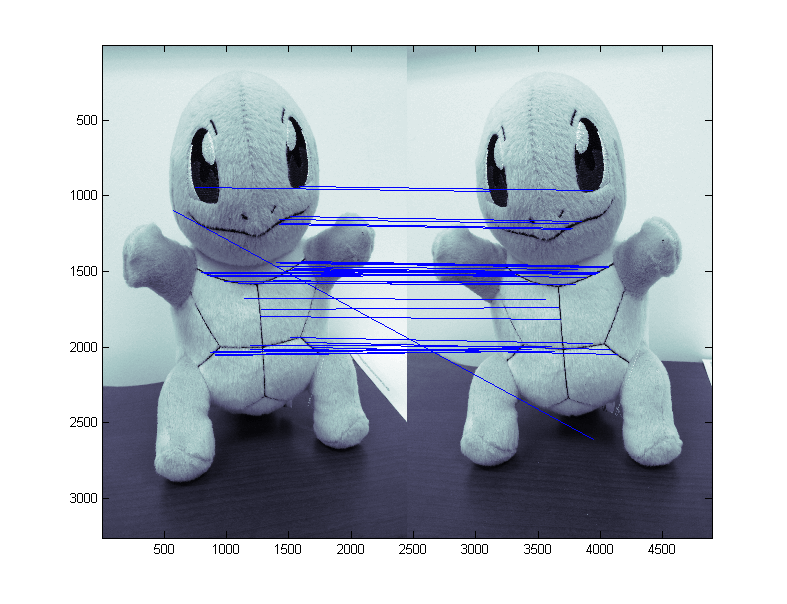
\includegraphics[height=5in]{squirtle_prob2Matches2.png}
\caption{Squirtle Images with matching points}
\label{p2d}
\end{figure}

\begin{figure}[H]
\centering
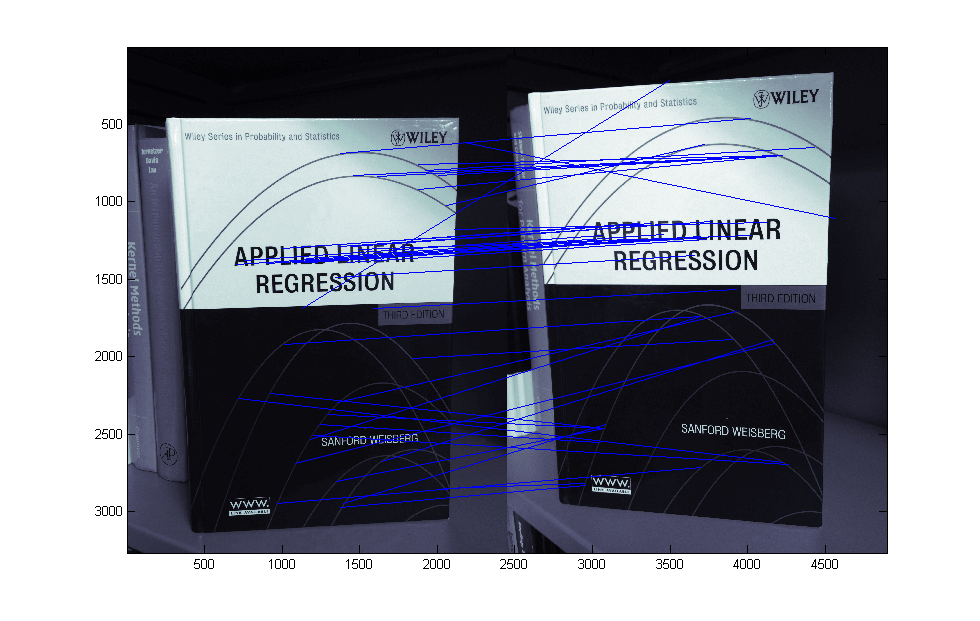
\includegraphics[height=5in]{book_prob2Matches2.png}
\caption{Textbook Images with matching points}
\label{p2e}
\end{figure}

\begin{figure}[H]
\centering
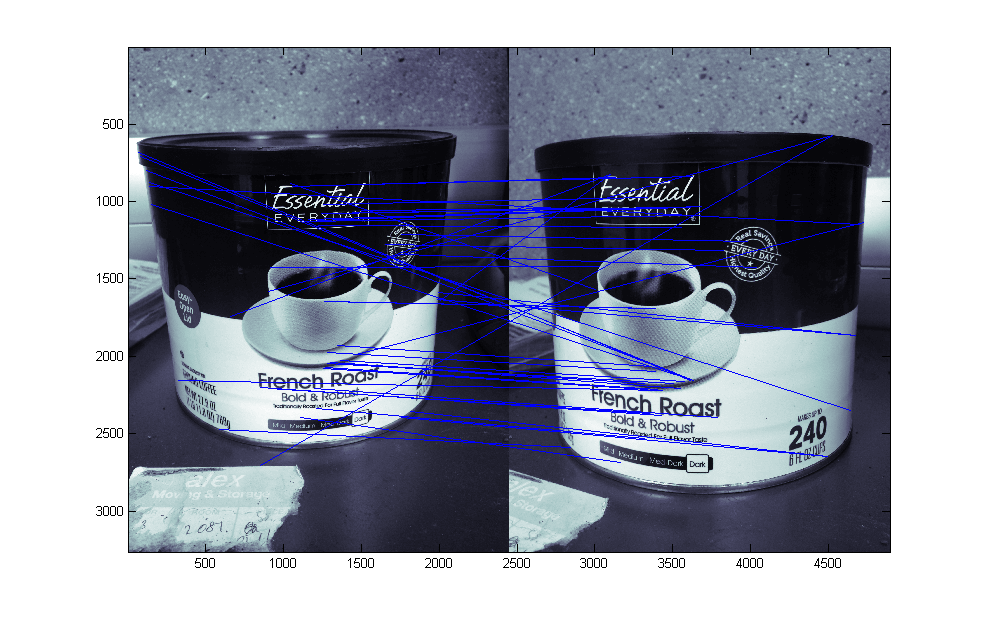
\includegraphics[height=5in]{coffeeCan_prob2Matches2.png}
\caption{Coffee Can Images with matching points}
\label{p2f}
\end{figure}

\newpage

\subsection*{Part B, SIFT points}

With the squirtle image epipoles for these points, they are nearly in the same spot. This would suggest that I did not move the camera much between the two images, which is consistent with what happened. With the coffee can image, there is a clear epipole in the right image but it is not clear in the left image where the epipole is located. This suggests that there were some inaccurate picks of points in this case.

\begin{figure}[H]
\centering
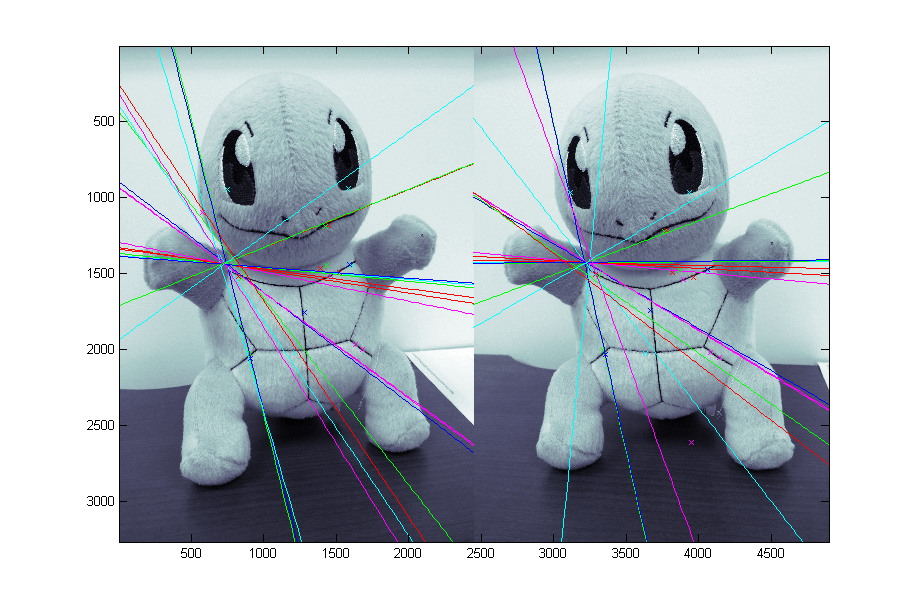
\includegraphics[height=3.5in]{squirtle_prob2Epipolar2.png}
\caption{Squirtle Image with Epipolar Lines and their points}
\label{p2g}
\end{figure}

\begin{figure}[H]
\centering
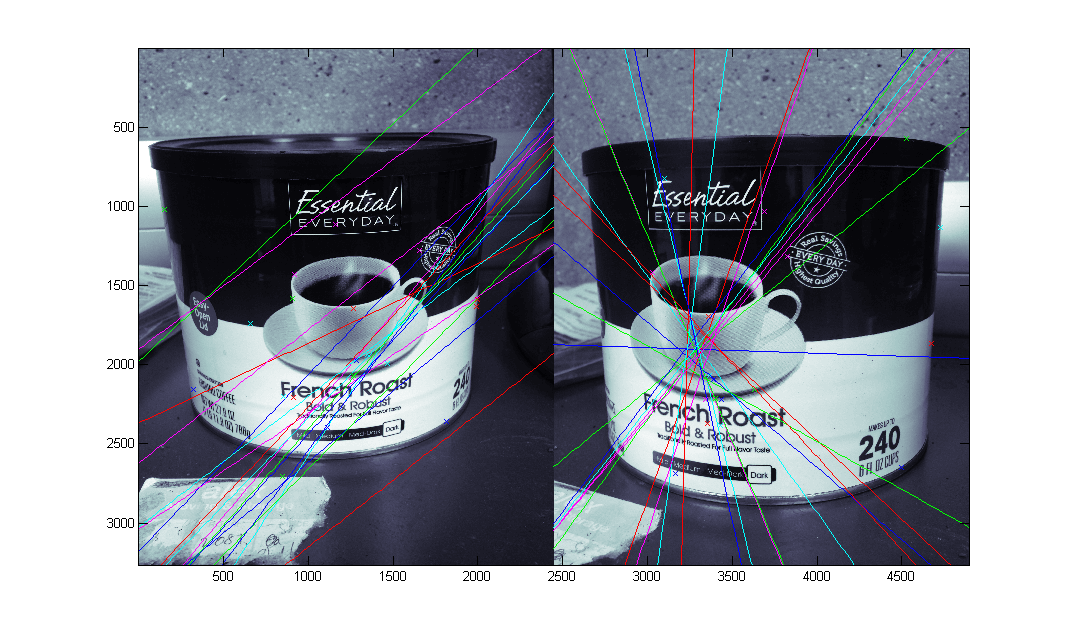
\includegraphics[height=3.5in]{coffeeCan_prob2Epipolar2.png}
\caption{Coffee Can Image with Epipolar Lines and their points}
\label{p2h}
\end{figure}

\newpage

\subsection*{Part C, SIFT points}

I repeated the procedure I did for my points to see the stability of F. \\
\\
For squirtle, the sum was 1.0191 and 4 computations of the F matrix were done. I decided to increase the number of points to see if that would make it more stable. After using 100 points in the RANSAC computation, the sum of the standard deviations of the entries was 0.0048 thus it had nearly the stability of my other method. \\
\\
For the textbook, the sum was near zero and 6 computations of the F matrix were done, thus it was more stable than my points.\\
\\
For the coffee can, the sum was near zero and 6 computations of the F matrix were done, thus it was more stable than my points. \\
\\
With these points, the estimates of F proved to be quite robust. As it turns out with the squirtle image, my hunch that when you add more points it becomes more robust proved correct. 

\subsection*{Code for Problem 2}

The code for this problem is attached as prob2script.m

\newpage

\section*{Problem 3}

After running everything, these are the two rotation matrices:
\[ \left( \begin{array}{ccc}
0.9920 & 0.1264 & $-3.7932e-5$\\
-0.1264 &  0.9920 & $-9.8549e-5$\\		
$-2.5167e-5$ & -0.0001 & -0.9999 \end{array} \right)\] 
\[ \left( \begin{array}{ccc}
-0.9920 & -0.1264 & $-1.1563e-4$\\
0.1264 &  -0.9920 & $1.8543e-5$\\		
$1.1704e-4$ & $-.7748e-6$ & -0.9999 \end{array} \right)\] 
The two position vectors are as follows\\
(7.6779e-5, 4.0003e-5,0.9999)
\\
(-7.6779e-5, -4.0003e-5,-0.9999)
\\
\\
According to these results, it appears that the camera was moved back (or forward) and then rotated to make the second image. This appears consisent with what the images look like. I would have expected slightly more movement in the $x,y$ direction though based on my perception of the image, but perhaps most of the translational movement was in the z direction. That is quite possible since there are only two camera positions we are considering. Figure 18 shows the image correspondences found through SIFT that were used to compute the above matrices and vectors.

\begin{figure}[H]
\centering
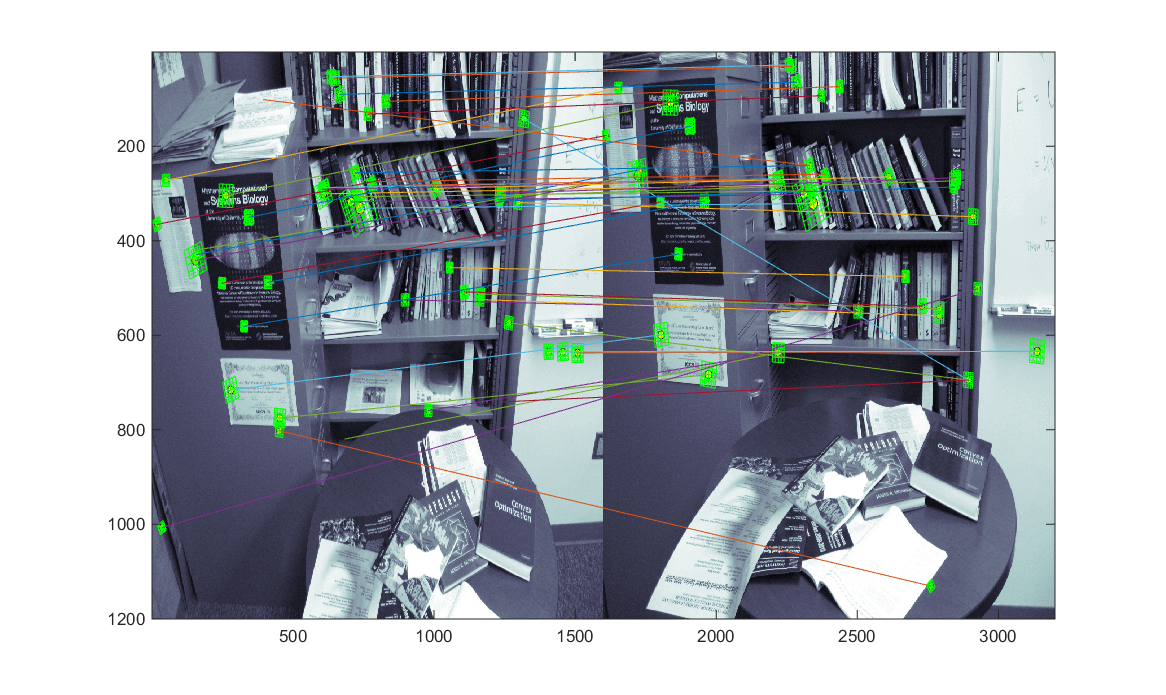
\includegraphics[height=4in]{prob3matches.png}
\caption{Image Correspondences}
\label{p3}
\end{figure}
      
The code to complete the problem is attached as prob3script.m   
        

\end{document}








